\section{Acceptance correction}
\label{sec:kstmm:ac}

The angular distribution of fully reconstructed and offline selected \BdToKstmm candidates 
is not representative of the angular distribution of \BdToKstmm events
which come from a proton-proton interaction.
This is because the process of reconstruction and selection introduces an acceptance
effect, both from the geometry of the \lhcb detector and from the reconstruction and selection
software. 
In order to perform an angular analysis, this acceptance effect must be corrected for.
There are two main approaches to including the acceptance in an angular analysis.
The acceptance can be parametrised and included in the signal \PDF and fitted to the data,
along with various external inputs to help constrain the parameters.
This approach has several benefits but it also introduces additional parameters into the fit.
Angular analyses that have used this approach include the \lhcb and \cdf measurements of $\Bd\to\jpsi\phi$~\cite{CDF:2011af,Aaij:1407836}.
As an alternative, the efficiency can be calculated in different regions of phase space to give each candidate a
weight proportional to the inverse of the efficiency,
\begin{align}
\omega(\ctl,\ctk,\phi)_i = \frac{1}{ \epsilon(\ctl,\ctk,\phi)_i } \, .
\end{align}
This method has the benefit of being separate from the result extraction, keeping the angular \PDF purely to describe the data. 
This is the method presented in this thesis and was the method used in the first two angular analyses of \BdToKstmm at \lhcb.

\subsection{Total acceptance effect on simulation}
\label{sec:kstmm:ac:effect}

Simulation was used to calculate the selection efficiency for \BdToKstmm candidates in different regions of phase space
by comparing the distribution of \BdToKstmm candidates as a function of the angular variables and \qsq
 before and after the complete selection has been applied.
The simulated events were generated as described in Section~\ref{sec:lhcb:soft} 
and corrected as described in Section~\ref{sec:kstmm:data:mccorr}.
The IP resolution and the particle identification corrections were applied before the selection. 
The distribution of the weights given to each of the simulated \BdToKstmm 
 candidates from the remaining data-simulation corrections is shown in Fig~\ref{fig:datamc:weight}.
\begin{figure}[tbp]
\centering
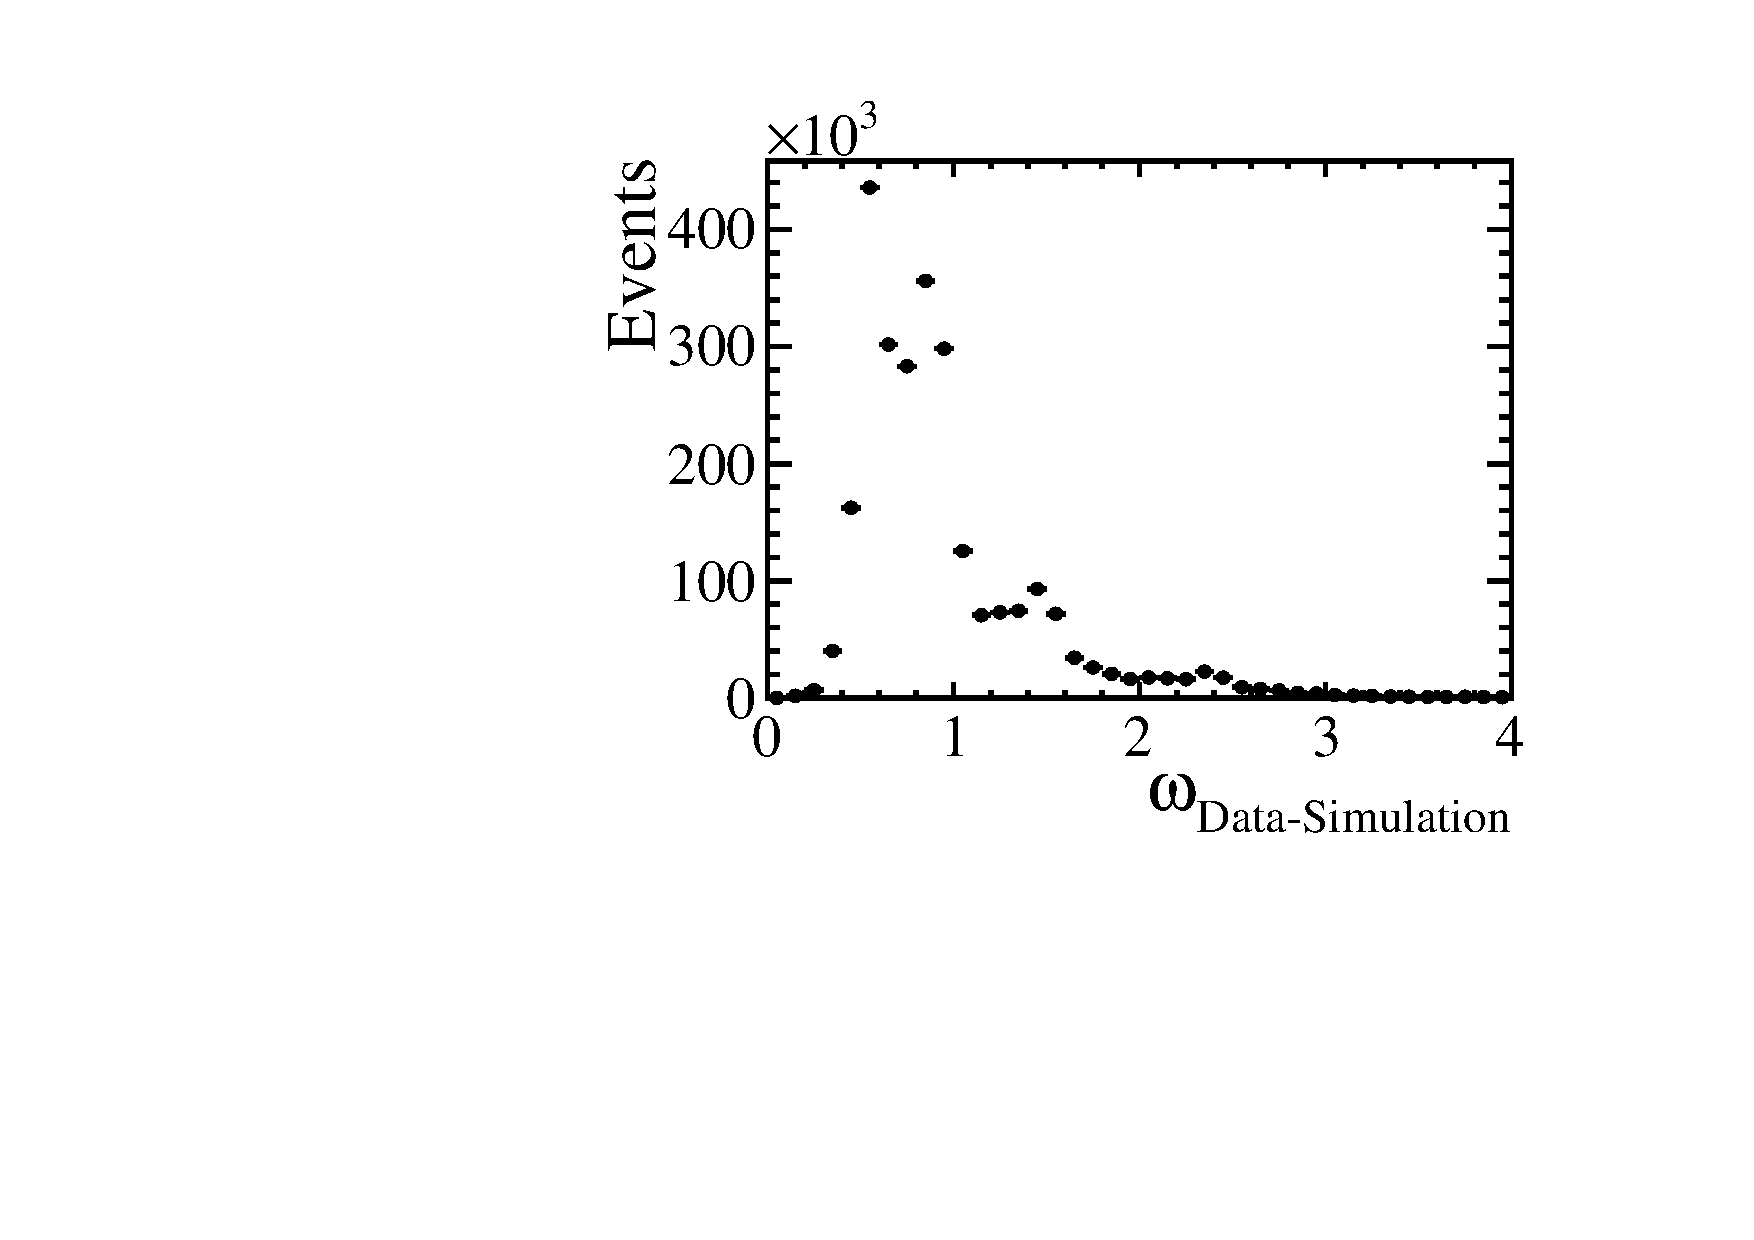
\includegraphics[width=0.48\columnwidth]{chapter5/figs/datamc/datamc_jpsikstar.pdf}
\caption{The distribution of weights to correct the simulated phase space \BdToKstmm candidates
 for known differences between the data and the simulation. ~\label{fig:datamc:weight} }
\end{figure}
The structure of four distinct peaks comes from the re-weighting for the event occupancy.

The angular distribution of fully reconstructed and selected phase space \BdToKstmm candidates
is given in Fig.~\ref{fig:phspeff}. 
\begin{figure}[tbp]
\centering
\subfigure[]{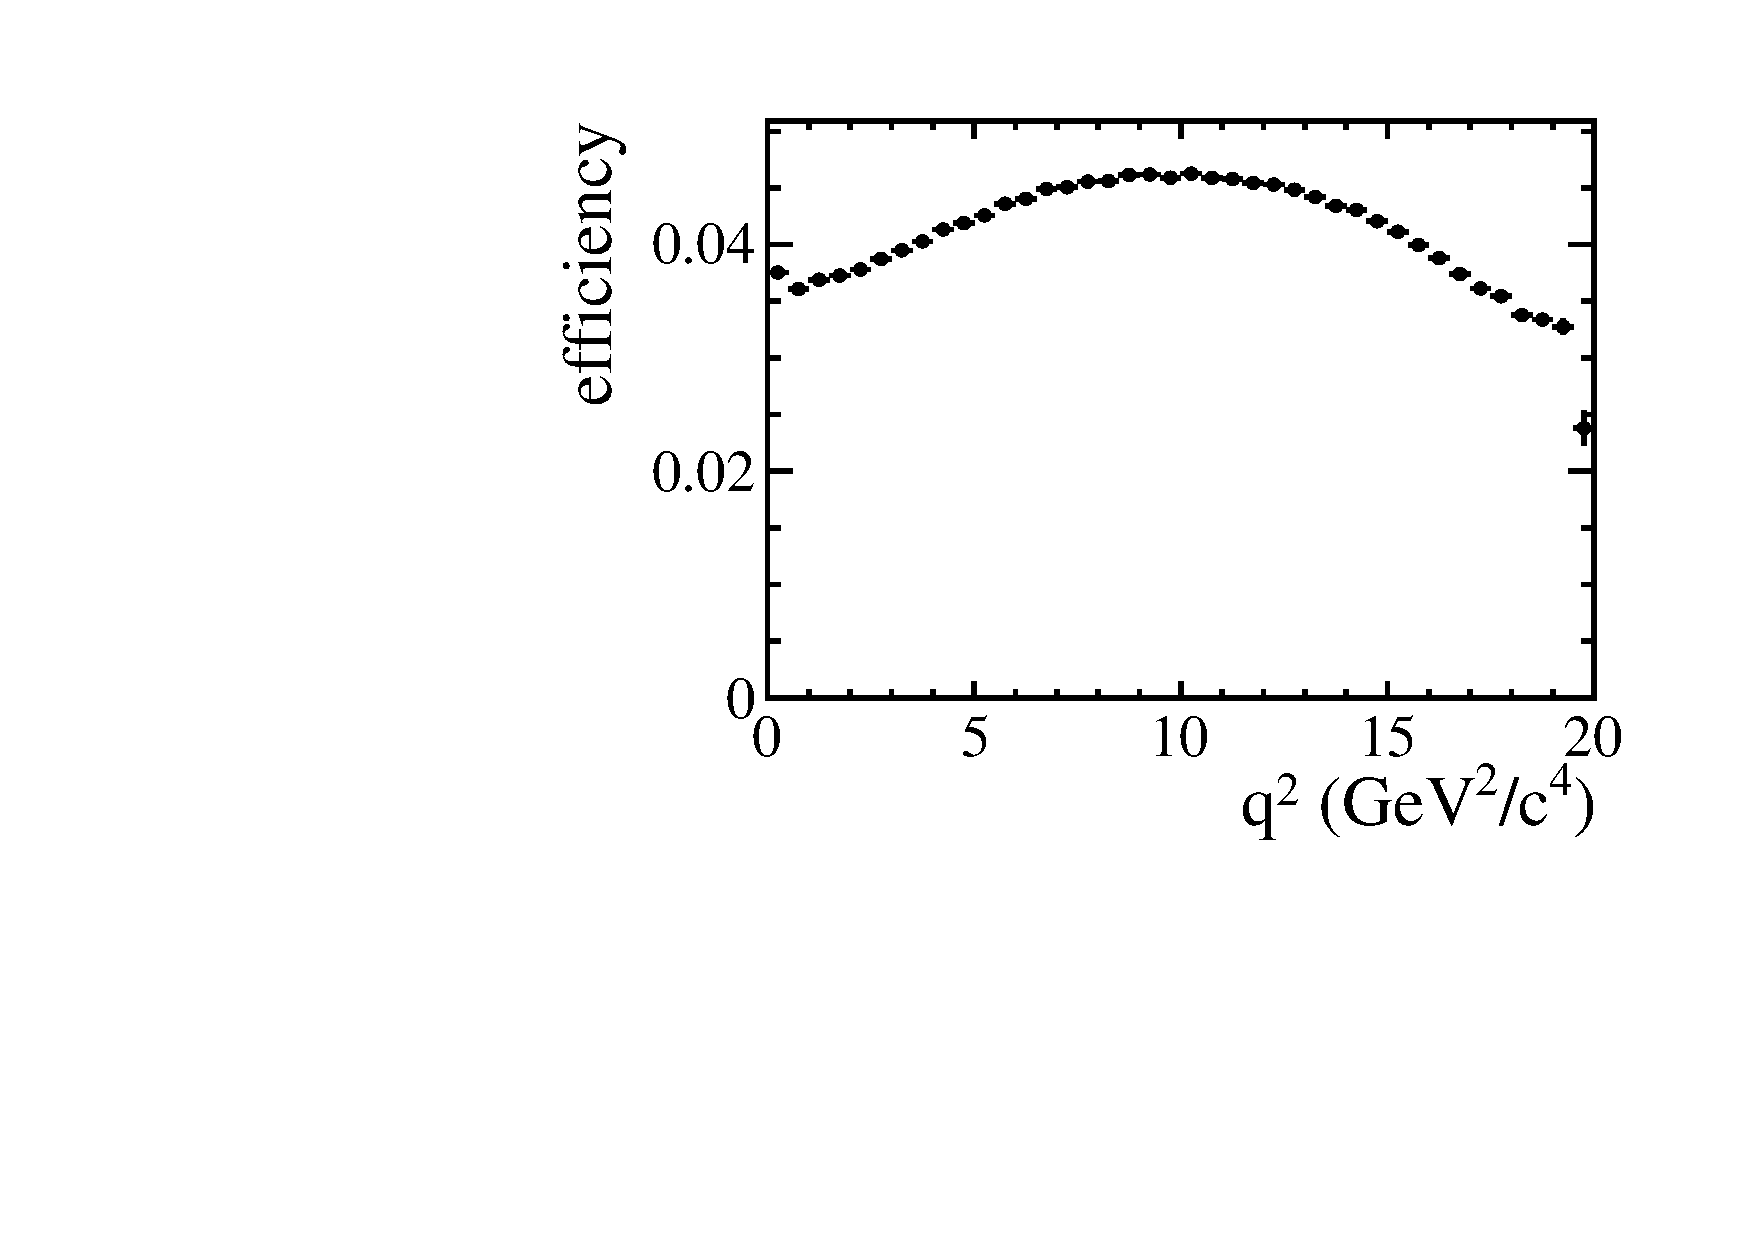
\includegraphics[width=0.48\columnwidth]{chapter5/figs/phsp_qsq_eff_dist.pdf}}
\subfigure[]{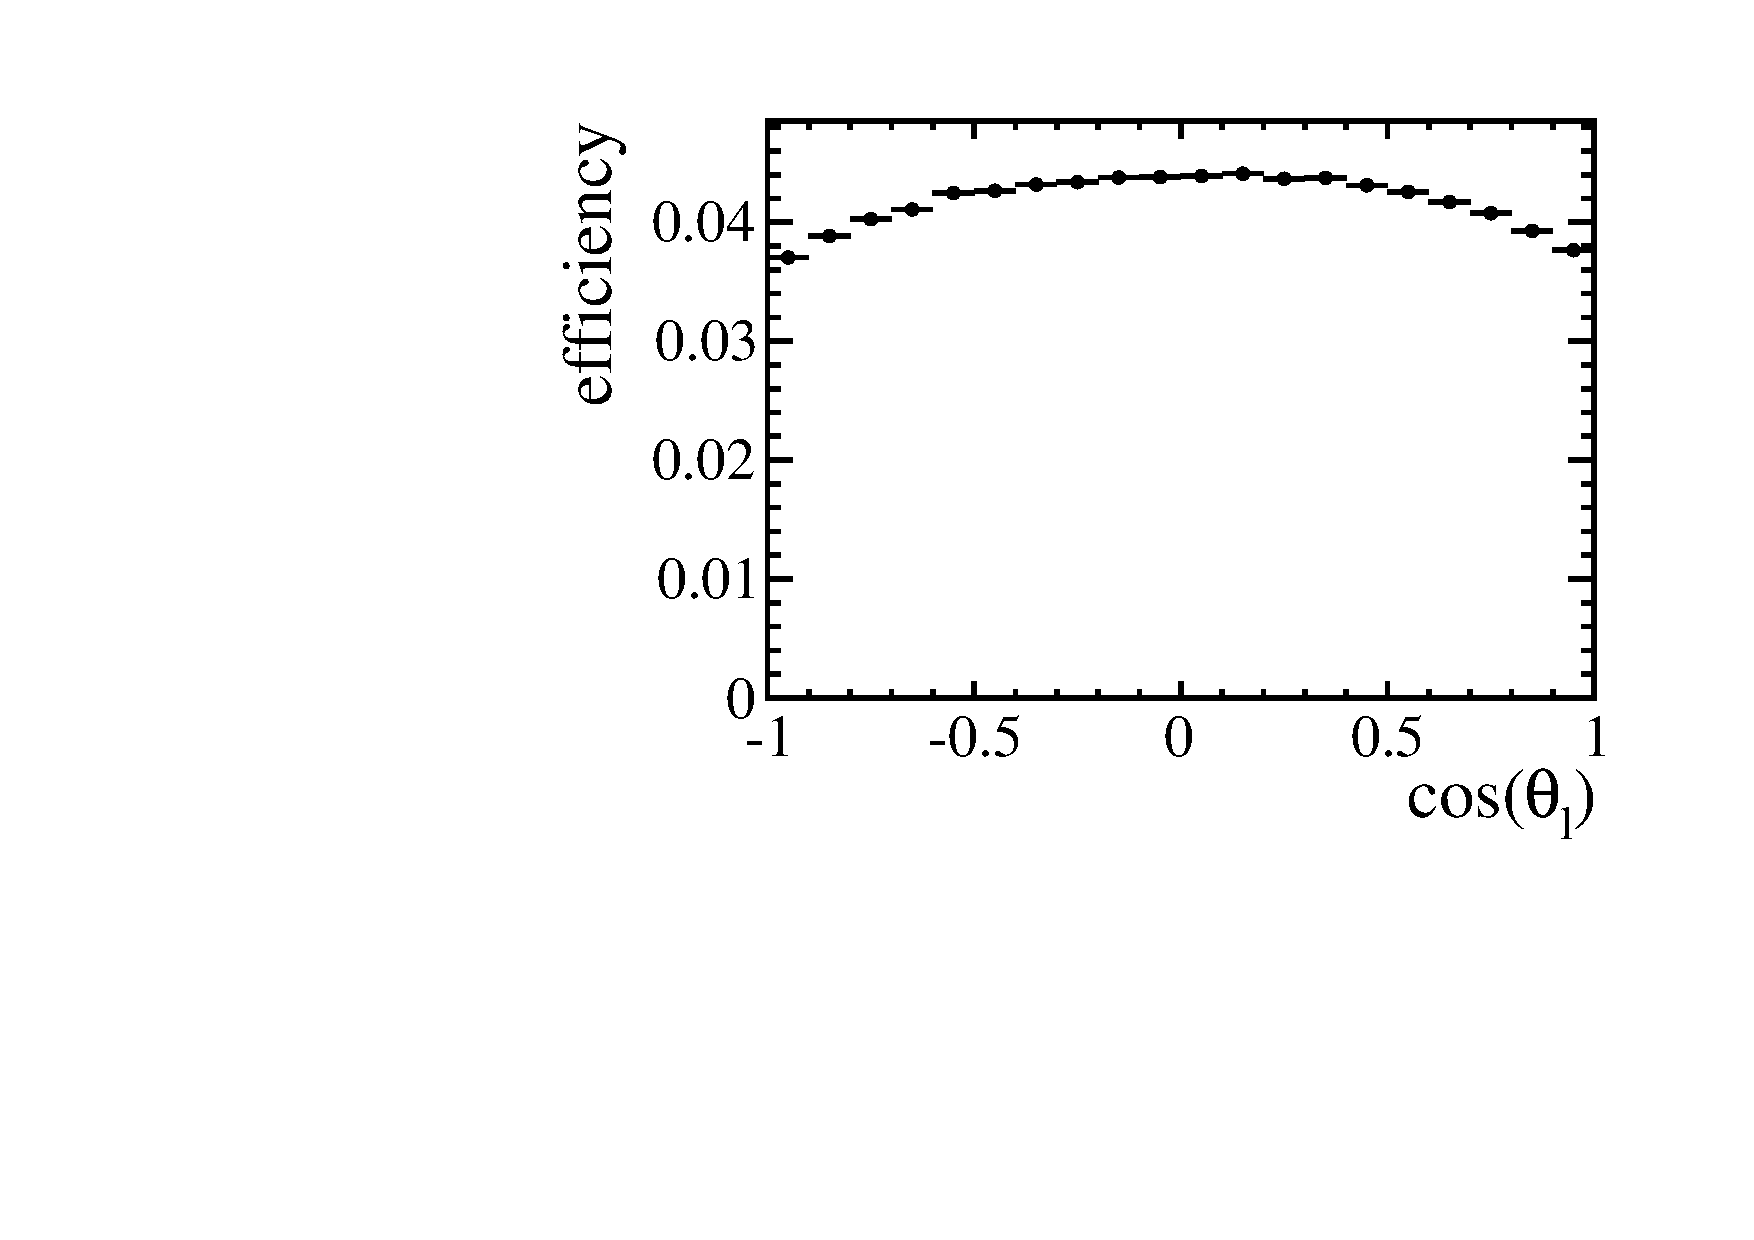
\includegraphics[width=0.48\columnwidth]{chapter5/figs/phsp_ctl_eff_dist.pdf}}
\subfigure[]{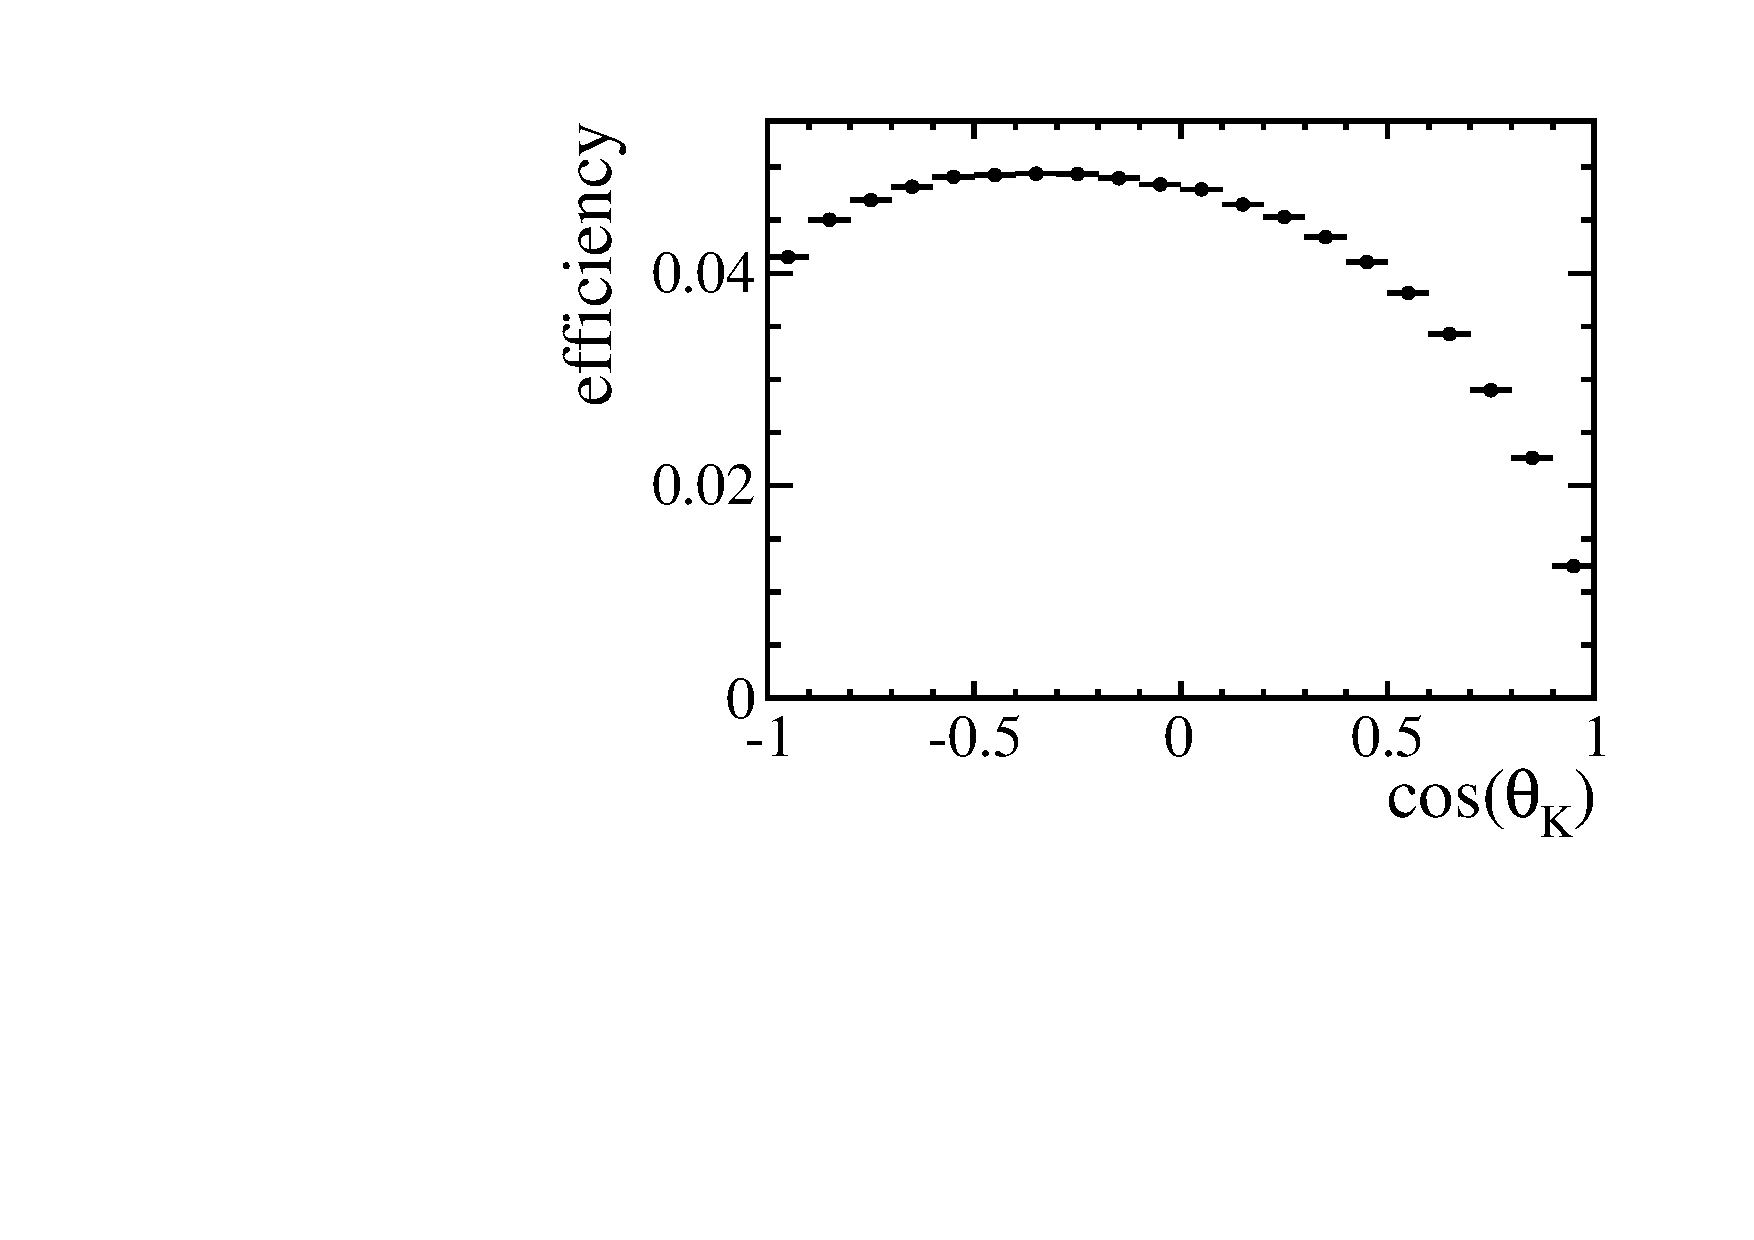
\includegraphics[width=0.48\columnwidth]{chapter5/figs/phsp_ctk_eff_dist.pdf}}
\subfigure[]{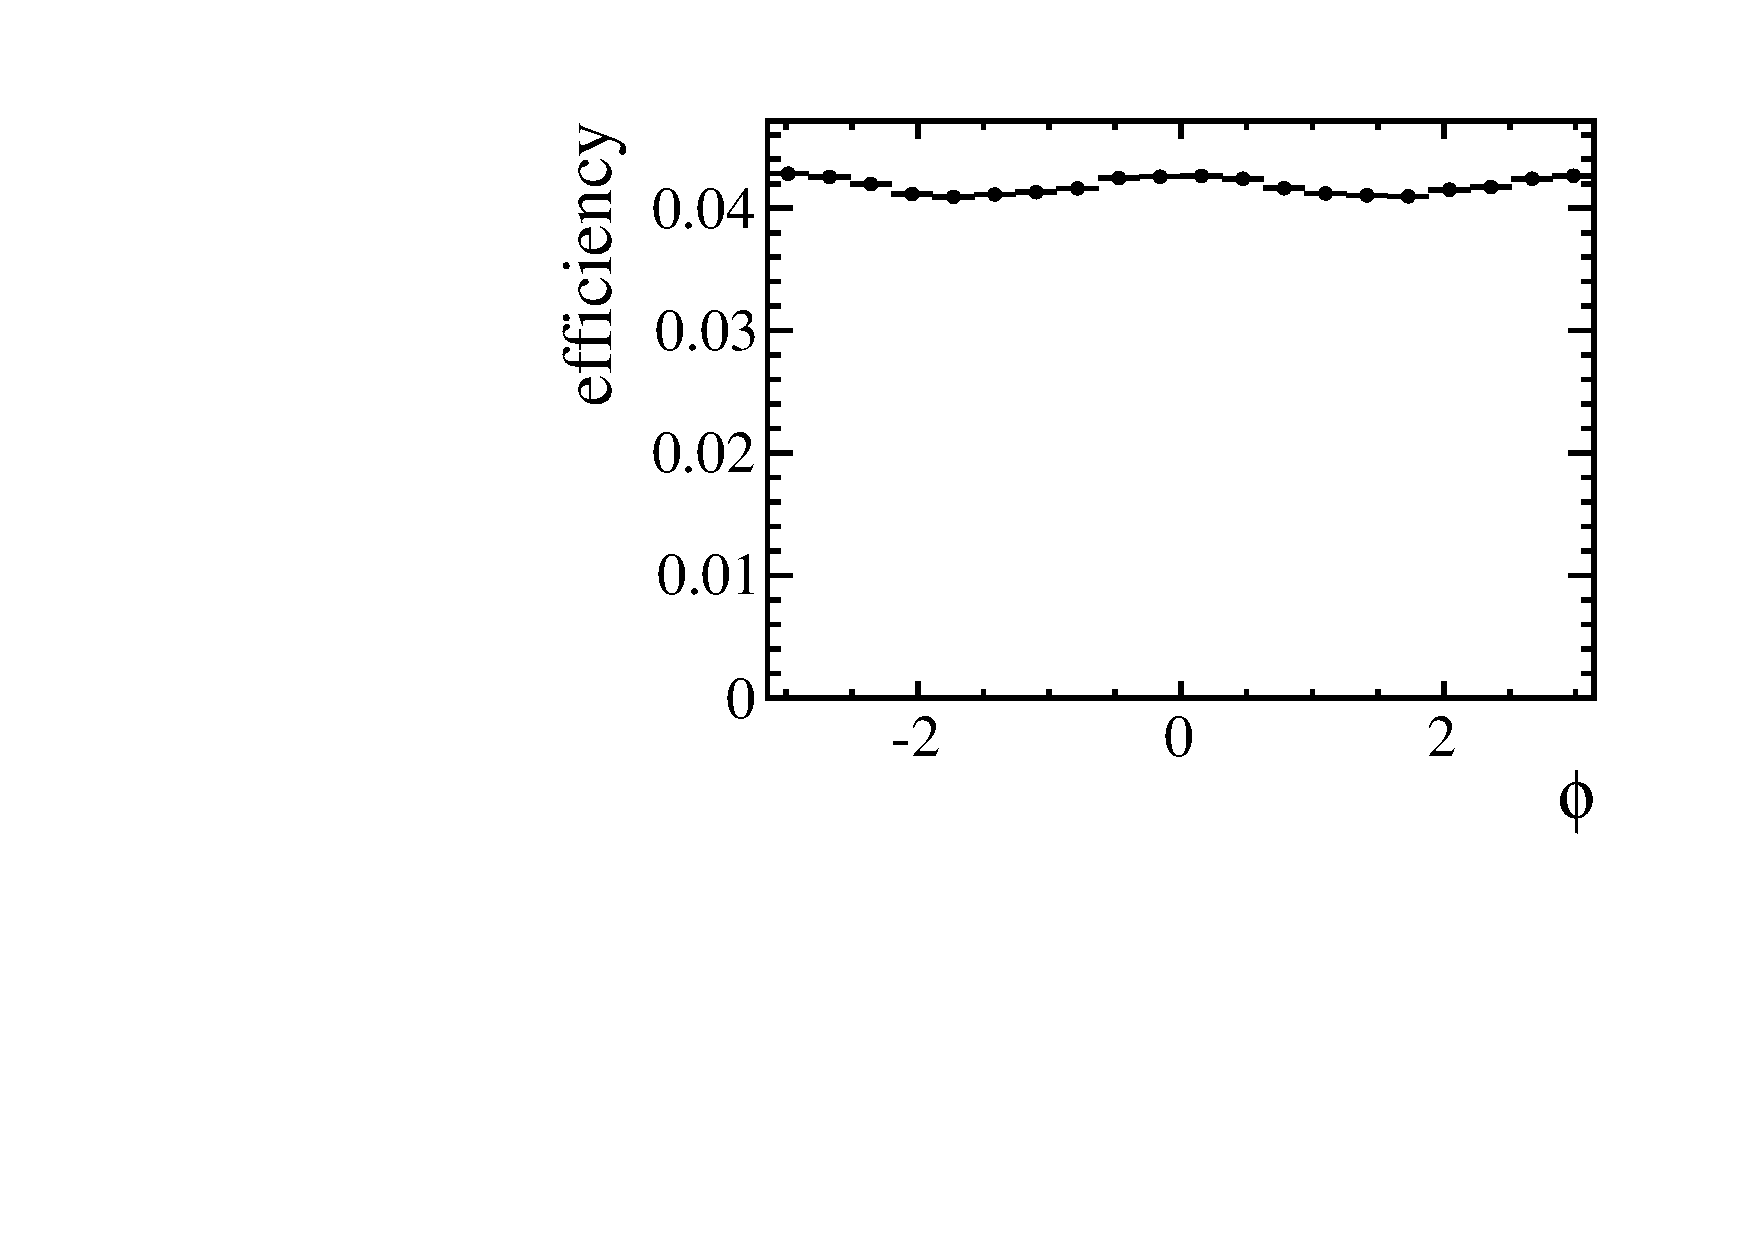
\includegraphics[width=0.48\columnwidth]{chapter5/figs/phsp_phi_eff_dist.pdf}}
\caption[The selection efficiency for \BdToKstmm on simulation]
{The efficiency for selected phase space simulated \BdToKstmm candidates as a function of (a) \qsq, (b) \ctl, (c) \ctk and (d) $\phi$. 
There is a reasonably symmetric acceptance in \ctl and an asymmetric acceptance effect in \ctk. 
The acceptance in \qsq varies across the full range and there is a very small acceptance effect in $\phi$.
 ~\label{fig:phspeff}}
\end{figure}
Is is possible to see the symmetric acceptance at high \ctl, due to 'backward-going' muons in the rest frame of the \Bd that have a very low momenta in the lab frame.
There is an asymmetric acceptance for \ctk from the same effect but the asymmetry is due to the difference in masses of the \kaon and the \pion. 
The different momentum spectra for the kaon and the pion is also affected by both the tracking efficiency and by the particle identification efficiency.
This is where most of the data/simulation corrections have a significant effect.

The total acceptance effect for a four-body decay is a function of the kinematic angles and invariant masses of the di-muon pair and the \kpi pair. 
The \psq window is assumed to be sufficiently small that there is no varying acceptance effect within it.
The angular analysis is performed in bins of \qsq requiring that the acceptance effect is corrected for on a finer level than the \qsq binning.


\subsection{A full 3D acceptance correction algorithm}
\label{sec:kstmm:ac:knnac}

One method of evaluating the efficiency as a function of phase space  is to count events before and after the selection
in fine bins of phase space.
This method was used in the first angular analysis of 0.38\invfb of data.
For an event at a particular point, the efficiency can be calculated by comparing the number of offline selected 
events with the number of generator level events `close' to that point : 
\begin{align}
\epsilon (\ctl, \ctk, q^2)_{r<R} = \frac{\offsel~(\delta d < R)  }{\genlvl~(\delta d < R)  } = \frac{n}{m}
\label{eq:eff}	
\end{align}
where $n$ is the number of weighted offline selected simulated events and $m$ is the number of generator level simulated events.
The distance $d$ is defined over the metric of the phase space and $R$ is the maximum distance within which events are chosen to contribute 
to the efficiency calculation.
The condition $\delta d < R$ defines a hyper-spheroid over the phase space.
The distance between event $i$ and event $j$, $\delta d_{ij}$, is given by
\begin{align}
\delta d_{ij} = \frac{1}{N_{\ctl}}( \ctl_i - \ctl_j  )^2 + \frac{1}{N_{\ctk}}( \ctk_i - \ctk_j) ^2 + \frac{1}{N_{\qsq}}( \qsq_i - \qsq_j) ^2 
\label{eq:distance}
\end{align}
where the normalisation factors, $(N_{\ctl}, N_{\ctk},N_{\qsq})$, are chosen such that the dimensions are each scaled between $[0,1]$. 
In order to collect events efficiently, a $k$-nearest neighbour algorithm was used to collect events in a small region of phase space. 

The error on the efficiency for a given bin is defined by the combination of the Poisson errors from $n$ and $m$, i.e.
\begin{align}
\sigma_{\epsilon} = \epsilon \times \sqrt{\frac{\sigma_n^2}{n^2} + \frac{1}{m}},
\end{align}
since the offline selection simulation is not a subset of the generation simulation.
The maximum radius $R$ is chosen such that the statistical error from the number of events within the hyper-spheroid is sufficiently small when compared to the size of the phase space. 
The average error and the average fractional error as a function of the radius of the hyper-spheroid is shown in Fig.~\ref{fig:errorvsradii}.
\begin{figure}[tbp]
\centering
\subfigure[]{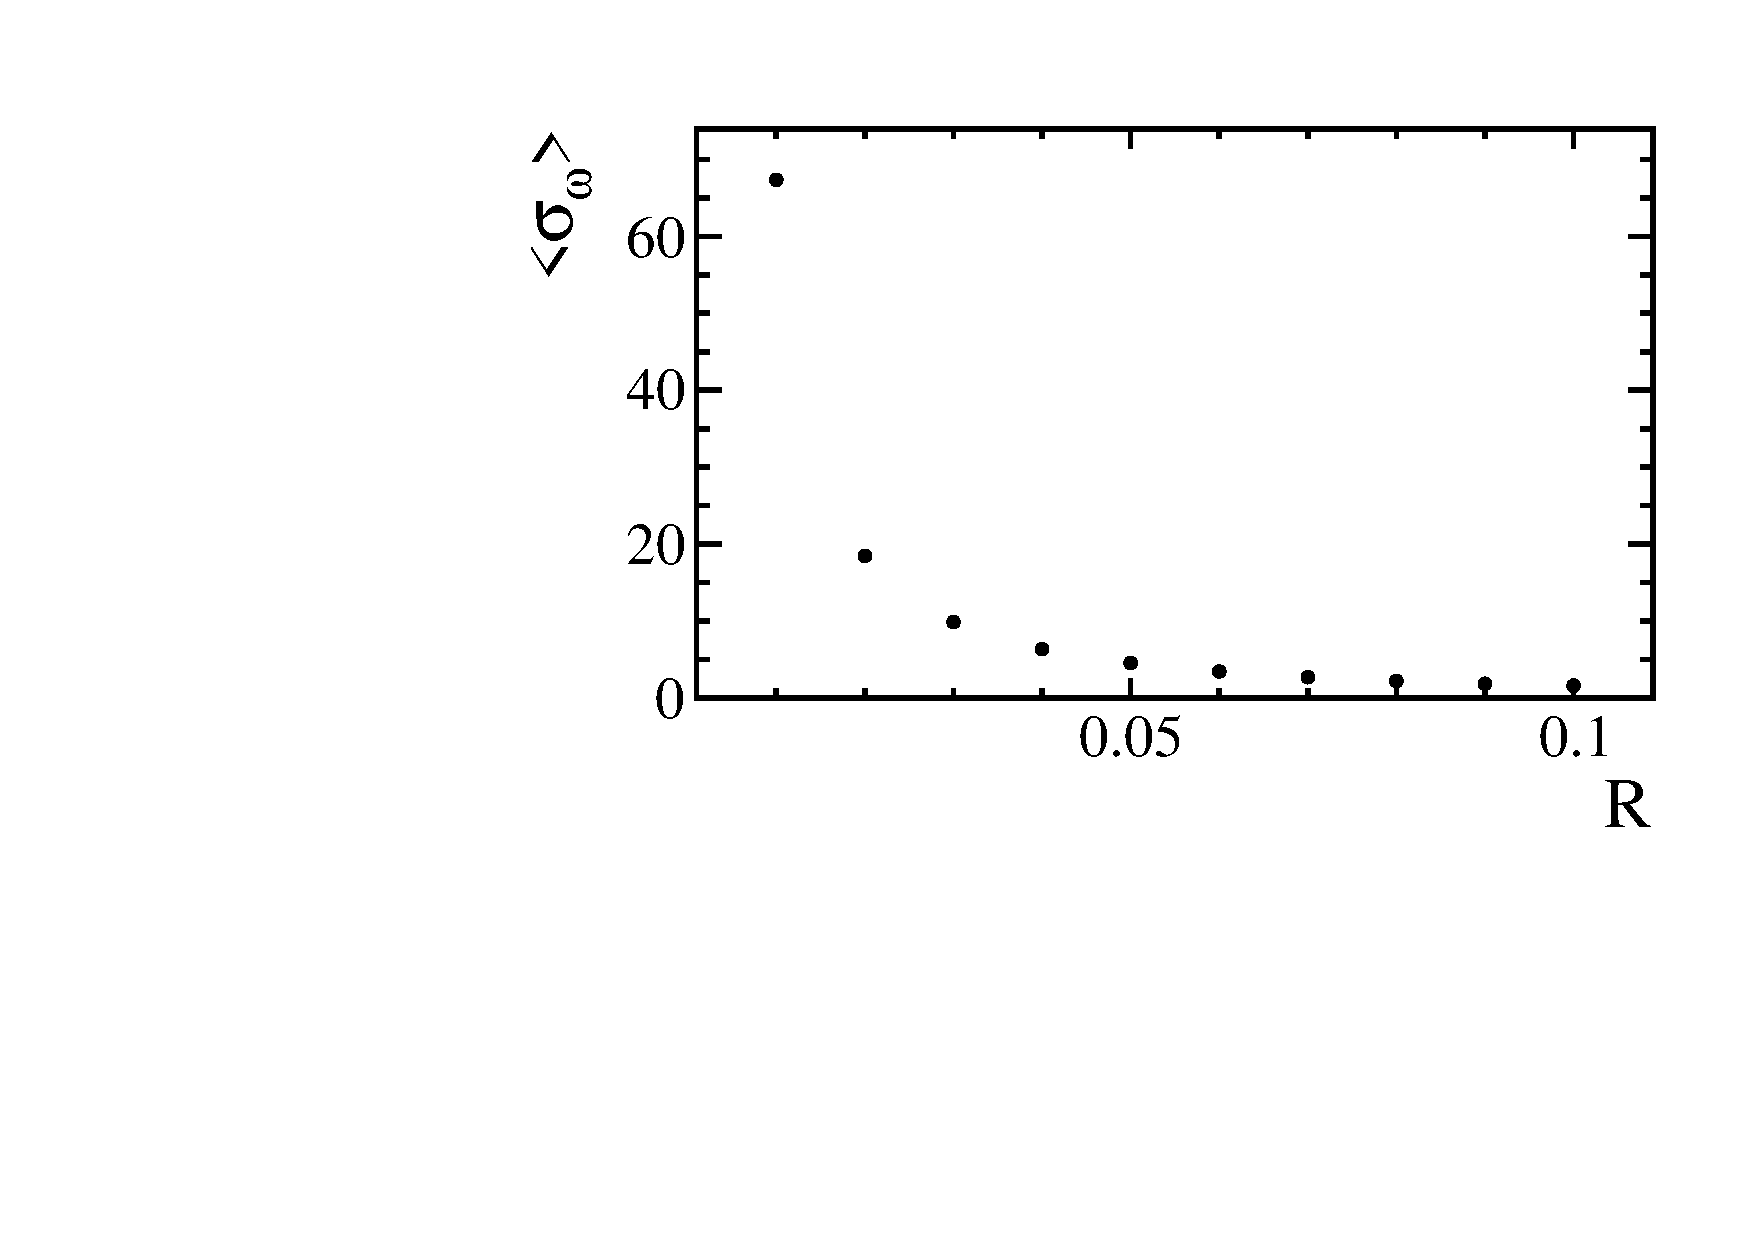
\includegraphics[width=0.48\columnwidth]{chapter5/figs/ac1/error_vs_radius.pdf}}
\subfigure[]{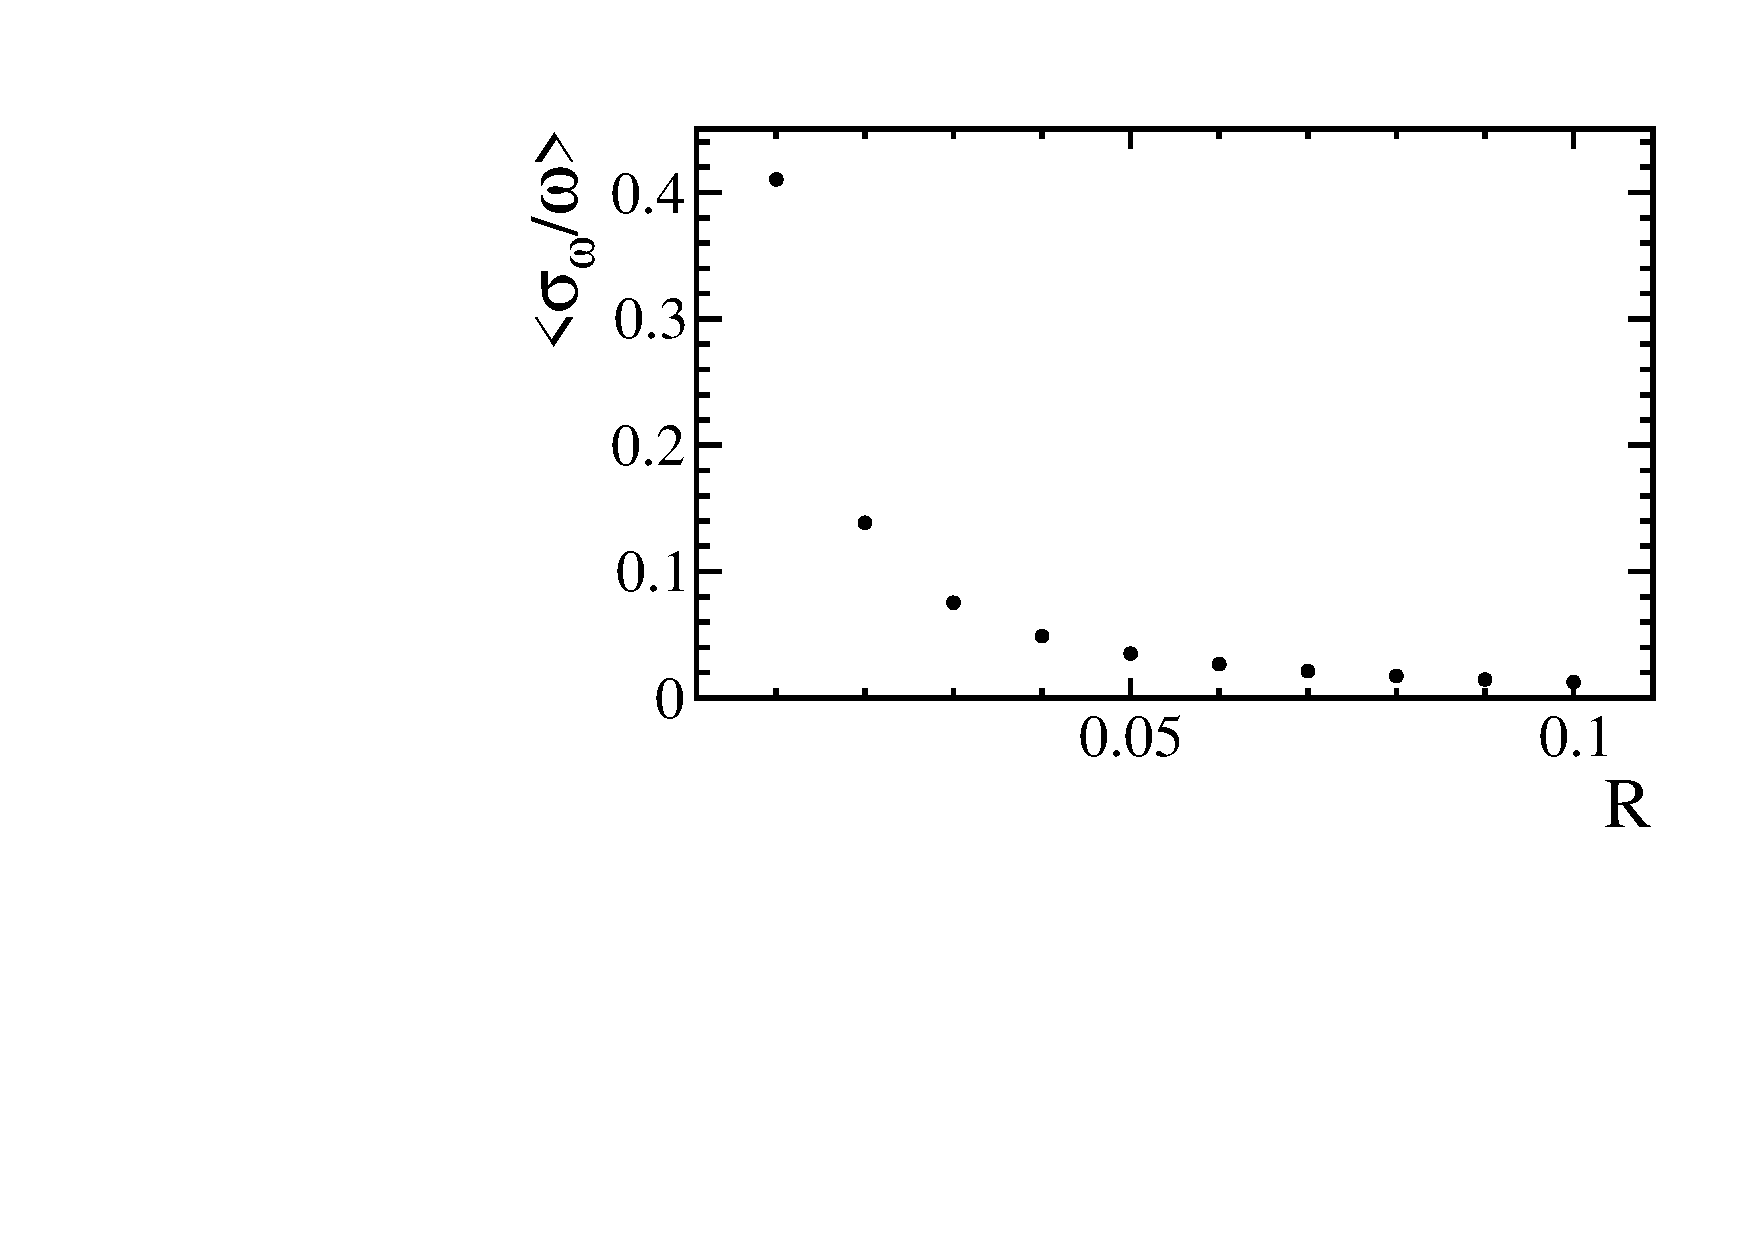
\includegraphics[width=0.48\columnwidth]{chapter5/figs/ac1/prop_error_vs_radius.pdf}}
\caption[The error on the acceptance correction weights.]
{ The average error (a) and the fractional error (b) on 150 weights for \BdToKstmm phase space simulated events for radii between 0.01 and 0.1. 
It is possible to see the $\sqrt{n^3}$ behaviour in the reduction of the error as more events are used to calculate the efficiency.
 ~\label{fig:errorvsradii} }
\end{figure}
The average error follows the expected Poisson behaviour but the fractional error is significant for radii of less than 0.02.

For the first angular analysis of 0.38\invfb of data, a radius of $R = 0.02$ was used to calculate an acceptance correction weight on an event-by-event basis.
This is chosen as a balance between contributing a large systematic error and retaining the accuracy on the correction.
The distribution of acceptance correction weights on data and the 
correlation between these weights and the angles are shown in Fig.~\ref{fig:ac1weights}.
\begin{figure}[tbp]
\centering
\subfigure[]{\includegraphics[width=0.48\columnwidth]{chapter5/figs/ac1/phasespace_weight_value.pdf}}
\subfigure[]{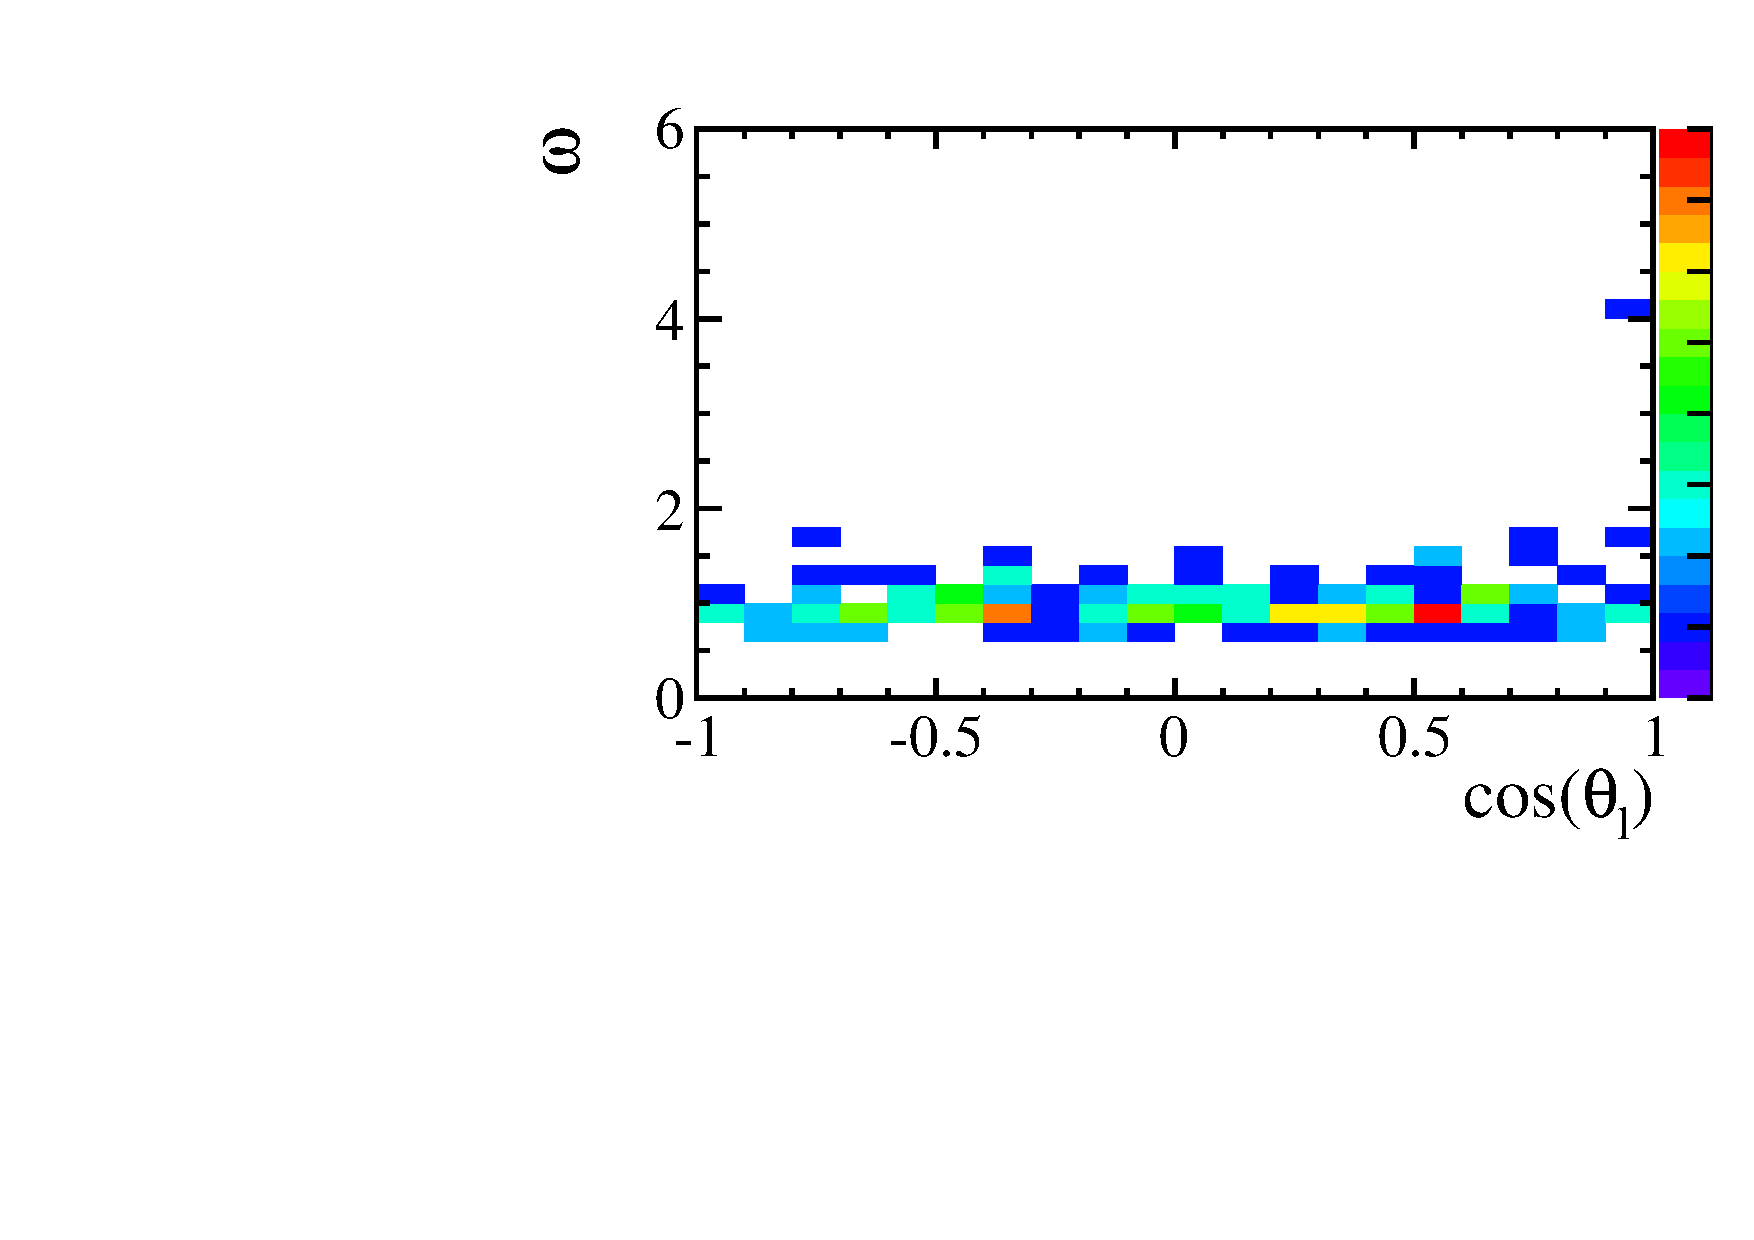
\includegraphics[width=0.48\columnwidth]{chapter5/figs/ac1/phasespace_weight_ctl.pdf}}
\subfigure[]{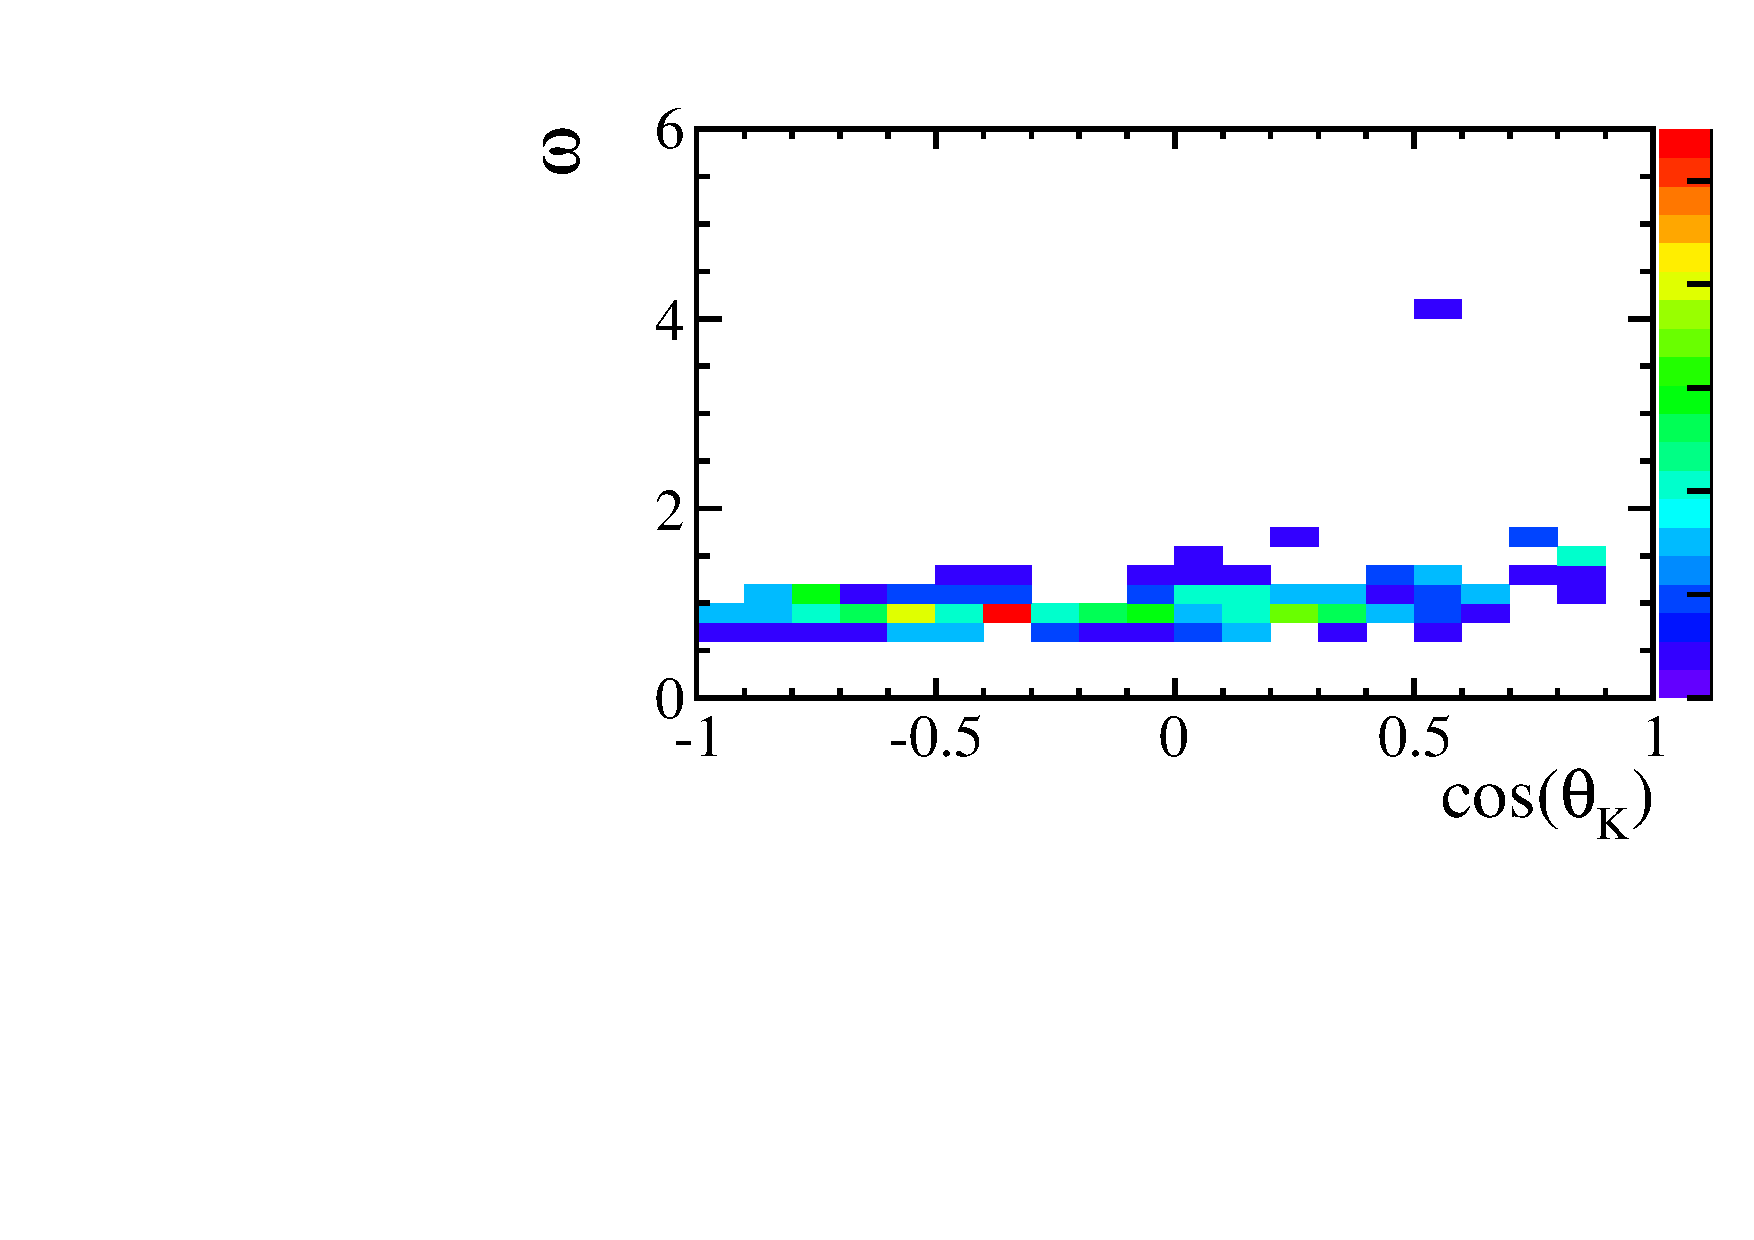
\includegraphics[width=0.48\columnwidth]{chapter5/figs/ac1/phasespace_weight_ctk.pdf}}
\caption[The weight distribution of acceptance corrected \BdToKstmm data.]
{ The distribution of weights for 150 phase space simulated \BdToKstmm events (a) and the correlation between 
the weights and \ctl (b) and \ctk (c). The weights are normalised such that the sum of weights is equal to the 
number of events. The high weights for extreme \ctk and \ctl can be seen. ~\label{fig:ac1weights} }
\end{figure}
It is possible to see that the weight values at extreme ($|\ctk|>0.8$) \ctk are higher than the weights in the centre.
The same effect can be seen in \ctl but to a lesser degree due to the integration over \qsq.
However, at low and high \qsq it is possible to see a variation of weights to accommodate the change in acceptance.

One limitation of the $k$-nearest-neighbour algorithm is 
that the error on the efficiency is entirely dominated 
by the number of offline selected simulated events at high \qsq.
If the data sample is binned more finely than the chosen collection radius $R$,
 then the `averaging effect' over the hyper-spheroid can be seen. 
In Fig.~\ref{fig:jpsikstardodgy}, an example of this can be seen in the large \BdToJpsiKstar sample.
\begin{figure}[tbp]
\centering
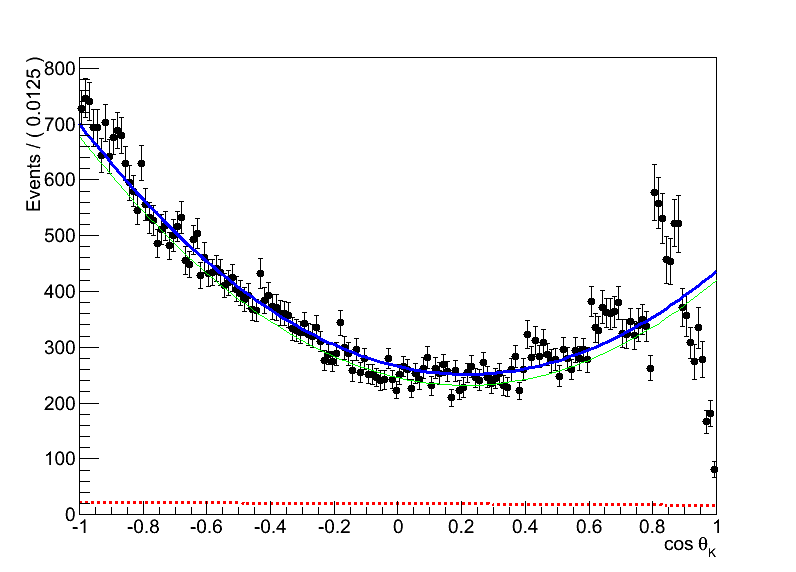
\includegraphics[width=0.48\columnwidth]{chapter5/figs/acceptance_variation_overbin.png}
\caption[ Weighted \BdToJpsiKstar events using a radius of $R = 0.05$. ]
{ Weighted \BdToJpsiKstar events using a radius of $R = 0.05$. 
The total expected number of events is shown in blue, along with the total expected number of signal events in green and the number of background events in red.
The effect of integrating over a rapidly varying efficiency is 
evident at high \ctk with a large statistics data sample. ~\label{fig:jpsikstardodgy} }
\end{figure}
A second limitation of the $k$-nearest-neighbour algorithm is the computational performance. 
The algorithm is at worst of order $\mathcal{O}(n)$ per event.
This can be simplified by only searching for neighbours in a small region of phase 
space, sufficient to encompass the subset of events within the radius $R$. 
As the number of events in the simulation has to scale with the size of the data, $n_{data}$,
 the overall scaling of the algorithm is $\mathcal{O}(n_{data}^2)$.
This, along with the required decrease in the systematic uncertainty on the efficiency calculation, 
necessitated the development of a more 
efficient acceptance algorithm for the angular analysis on the full 2011 dataset.

\subsection{A factorised acceptance correction algorithm}
\label{sec:kstmm:ac:facac}

In order to reduce the error on the acceptance correction beyond the reduction in statistical error for the full 2011 dataset, a factor of $1/\sqrt{3}$ was required to compensate for the threefold increase in data.
One solution to this issue, along with reducing the $\mathcal{O}(m^2)$ scaling of the $k$-nearest neighbour algorithm, 
is to model the distribution of events before and after selection using a \PDF.
The error on the fitted PDFs at a point in phase space is smaller than the error on a bin of $k$ events because 
the whole dataset is used to evaluate the efficiency.
%and PDFs, once fitted, can be evaluated at each point in phase space quickly.

In general, the efficiency function is not analytical so the choice of PDF to model the efficiency is entirely empirical.
The efficiency can be calculated at a particular point in phase space,
\begin{align}
\epsilon(\ctl, \ctk, \phi, \qsq) = \frac{n}{m} \times \frac{ S( \ctl, \ctk, \phi, \qsq ) }{ G( \ctl, \ctk, \phi, \qsq )  }  \, ,
\end{align}
where $S$ is the \PDF modelling the selected data and $G$ is the \PDF modelling the generator level data.
 The PDFs are normalised by the weighted number of events in the selected sample ($n$) divided by the number of generator level events ($m$).

Maximum use of the simulated events to give a large reduction in the error can be made by factorising the efficiency in the form,
\begin{align}
\epsilon(\ctl, \ctk, \phi,\qsq)  = \epsilon(\ctl)\times\epsilon(\ctk)\times\epsilon(\phi)\times\epsilon(\qsq) \, .
\end{align}
This factorisation is in general not possible due to the fact that there is a correlation between the angles and \qsq.
The efficiency for each of the angles for offline selected simulated phase space \BdToKstmm events 
 in a low \qsq bin are given in Fig.~\ref{fig:phspeff2d}. 
\begin{figure}[tbp]
\centering
\subfigure[\ctl v.s. \ctk]{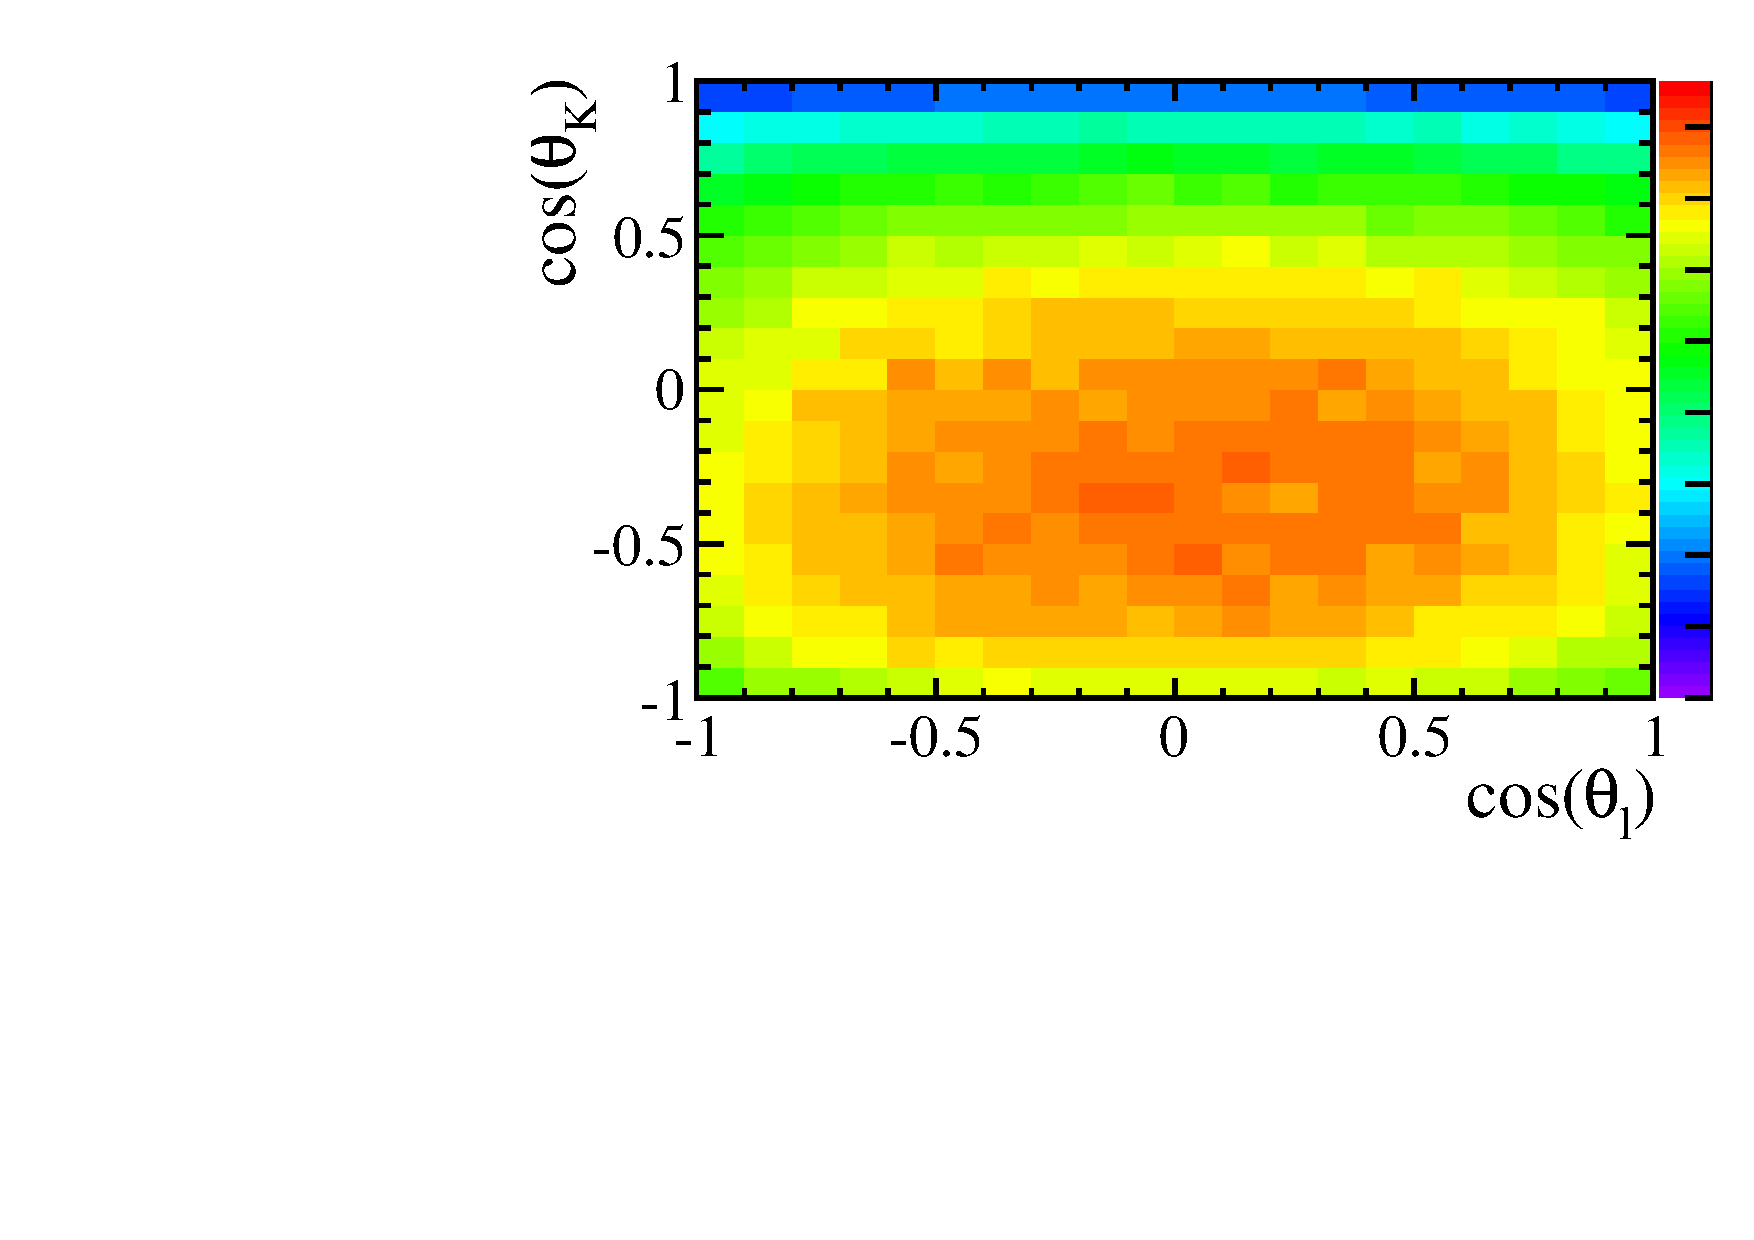
\includegraphics[width=0.48\columnwidth]{chapter5/figs/phsp_ctl_ctk_sel_dist.pdf}}
\subfigure[\ctl v.s. $\phi$]{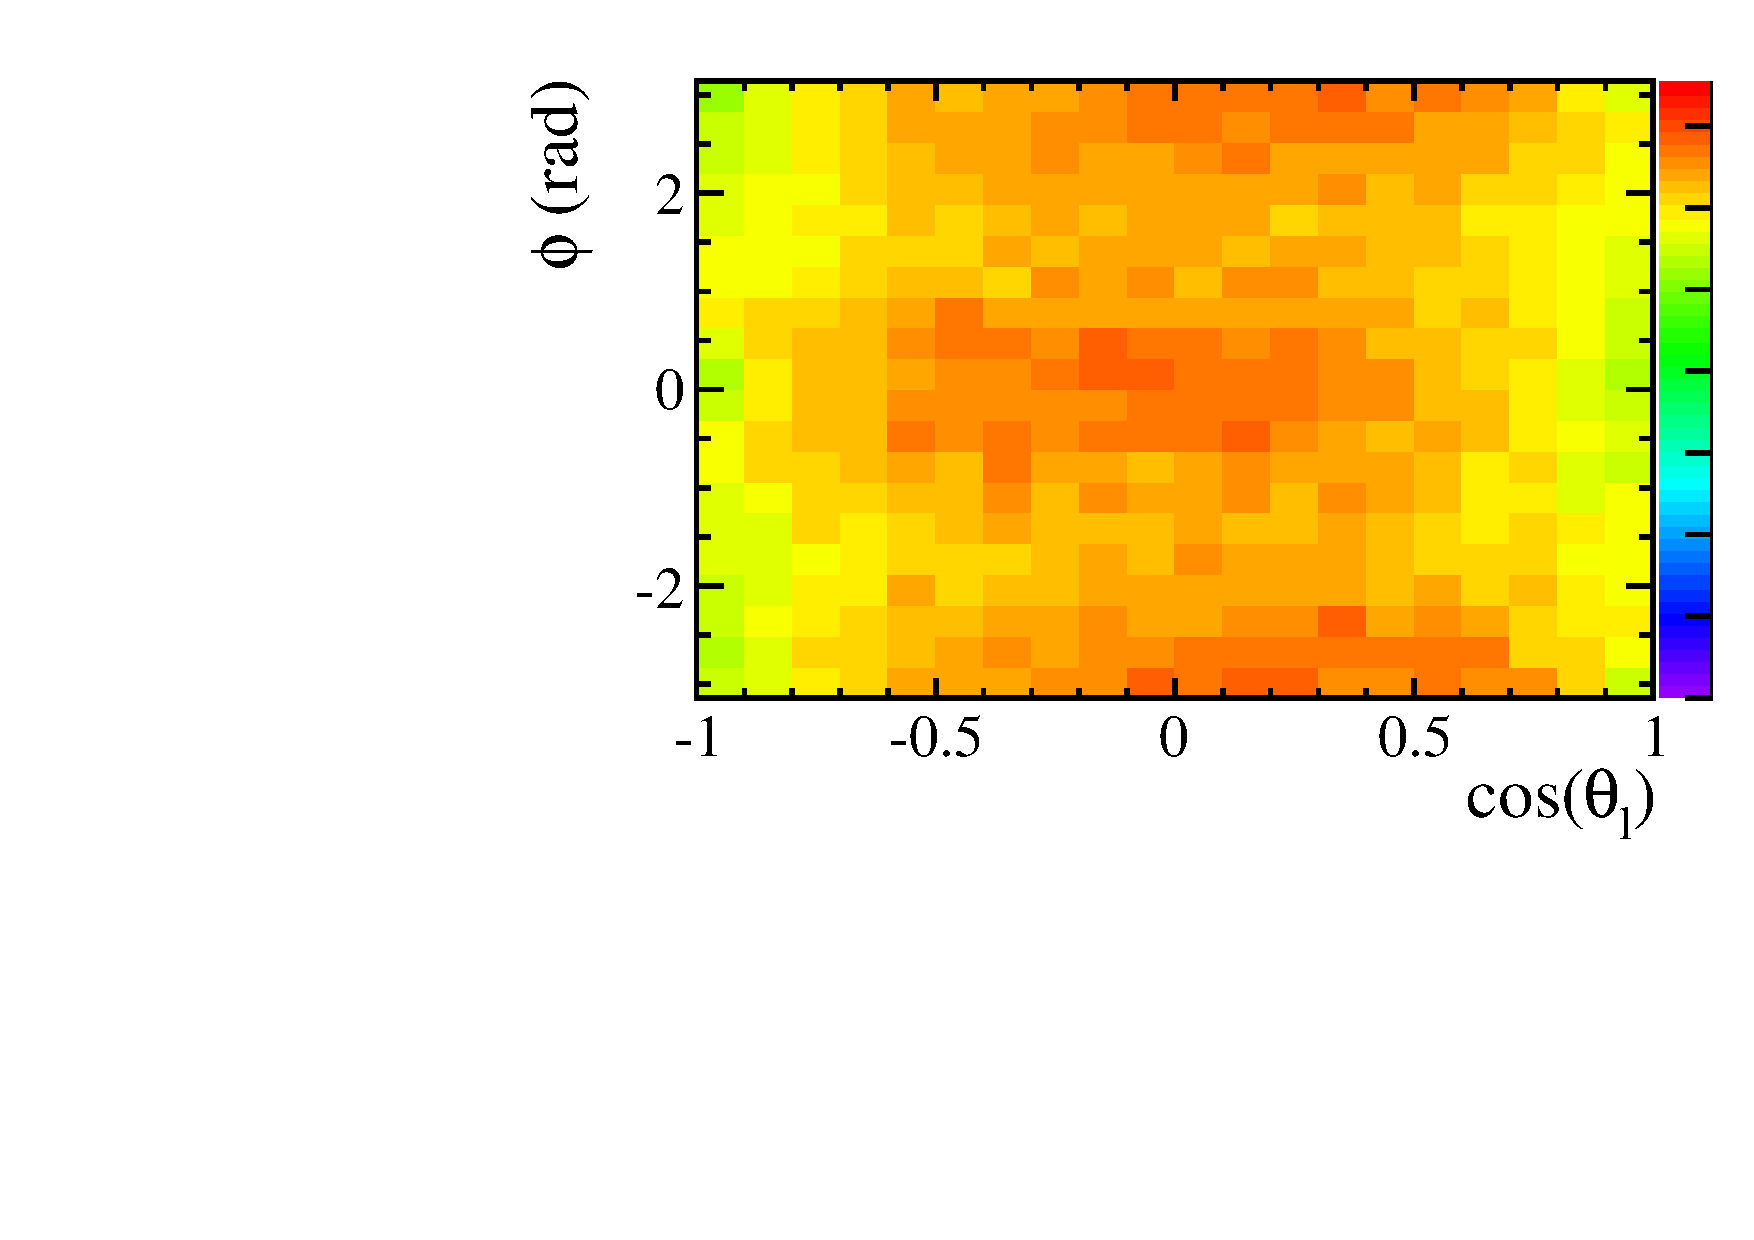
\includegraphics[width=0.48\columnwidth]{chapter5/figs/phsp_ctl_phi_sel_dist.pdf}}
\subfigure[\ctk v.s. $\phi$]{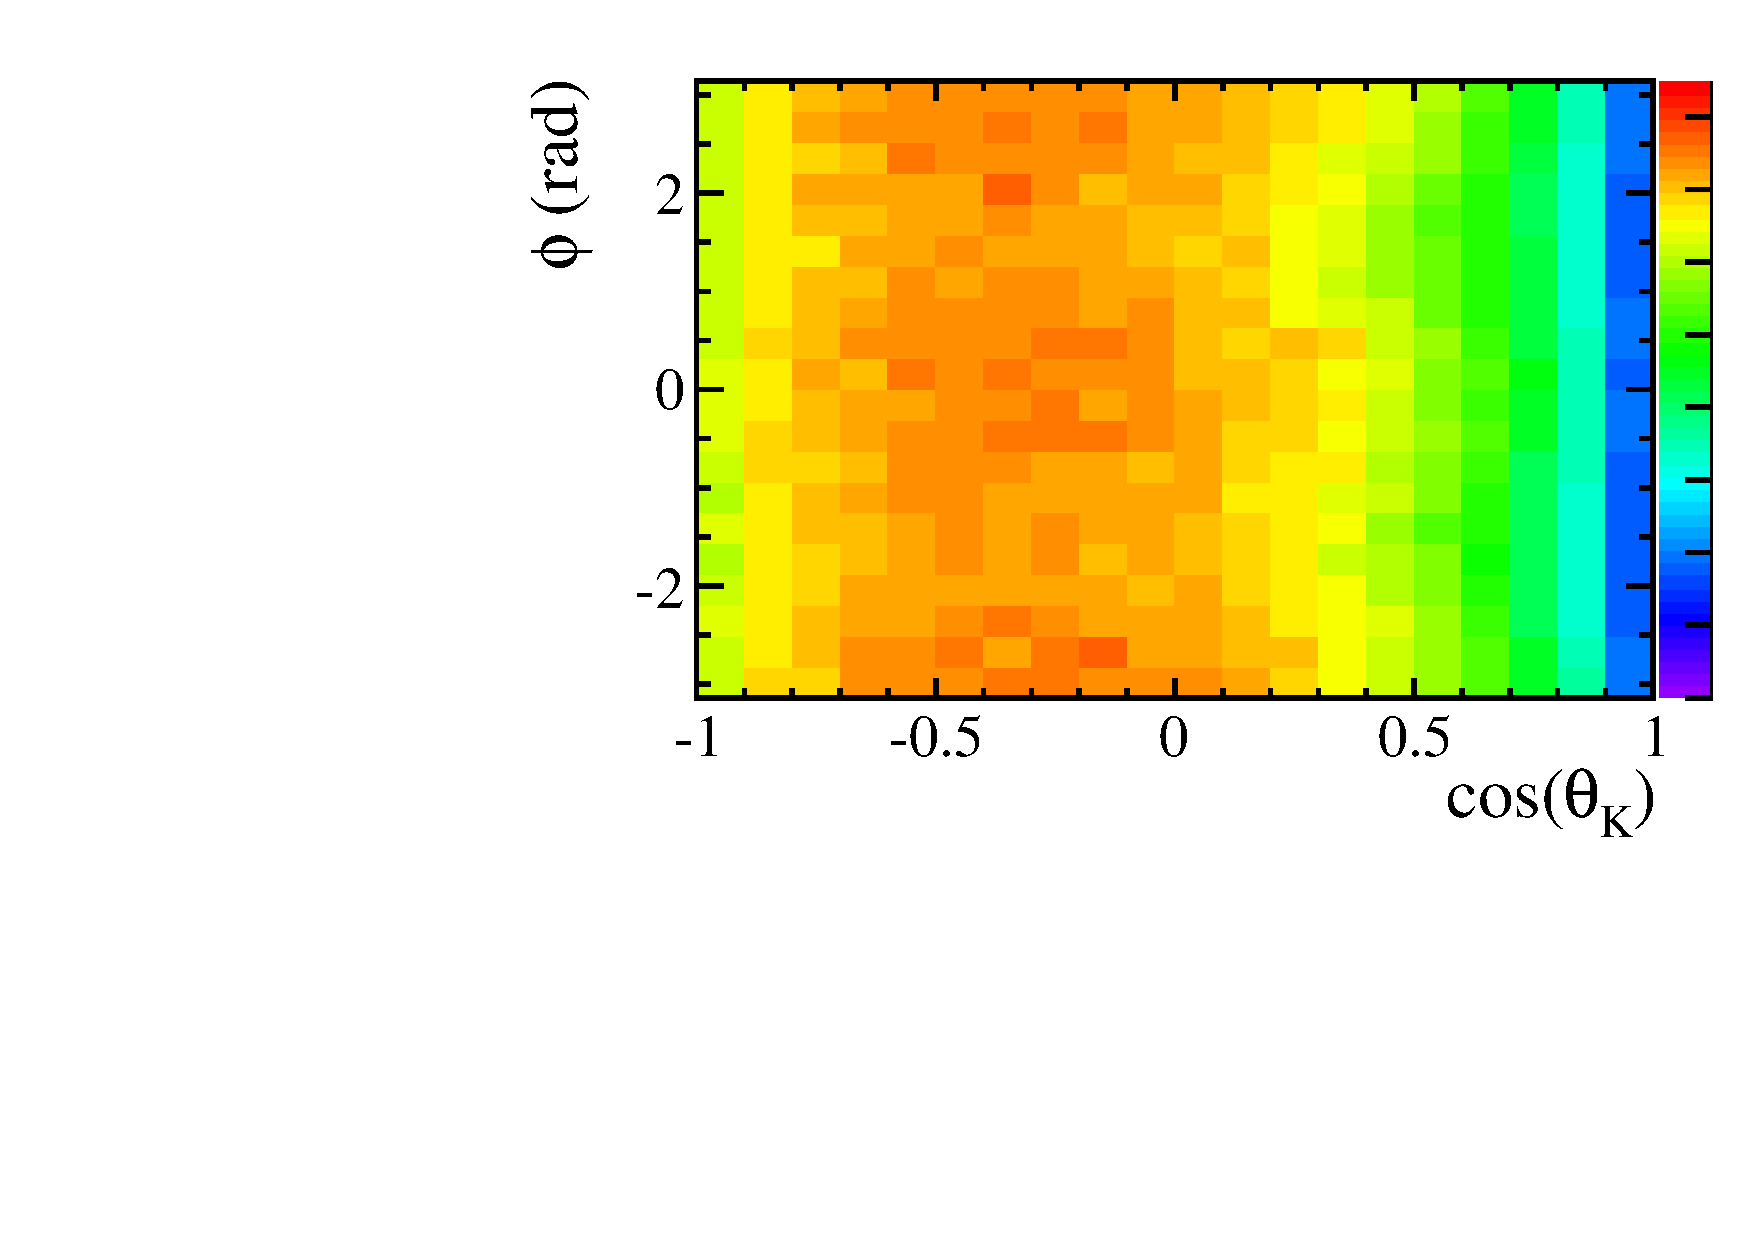
\includegraphics[width=0.48\columnwidth]{chapter5/figs/phsp_ctk_phi_sel_dist.pdf}}
\subfigure[\ctl v.s. \qsq]{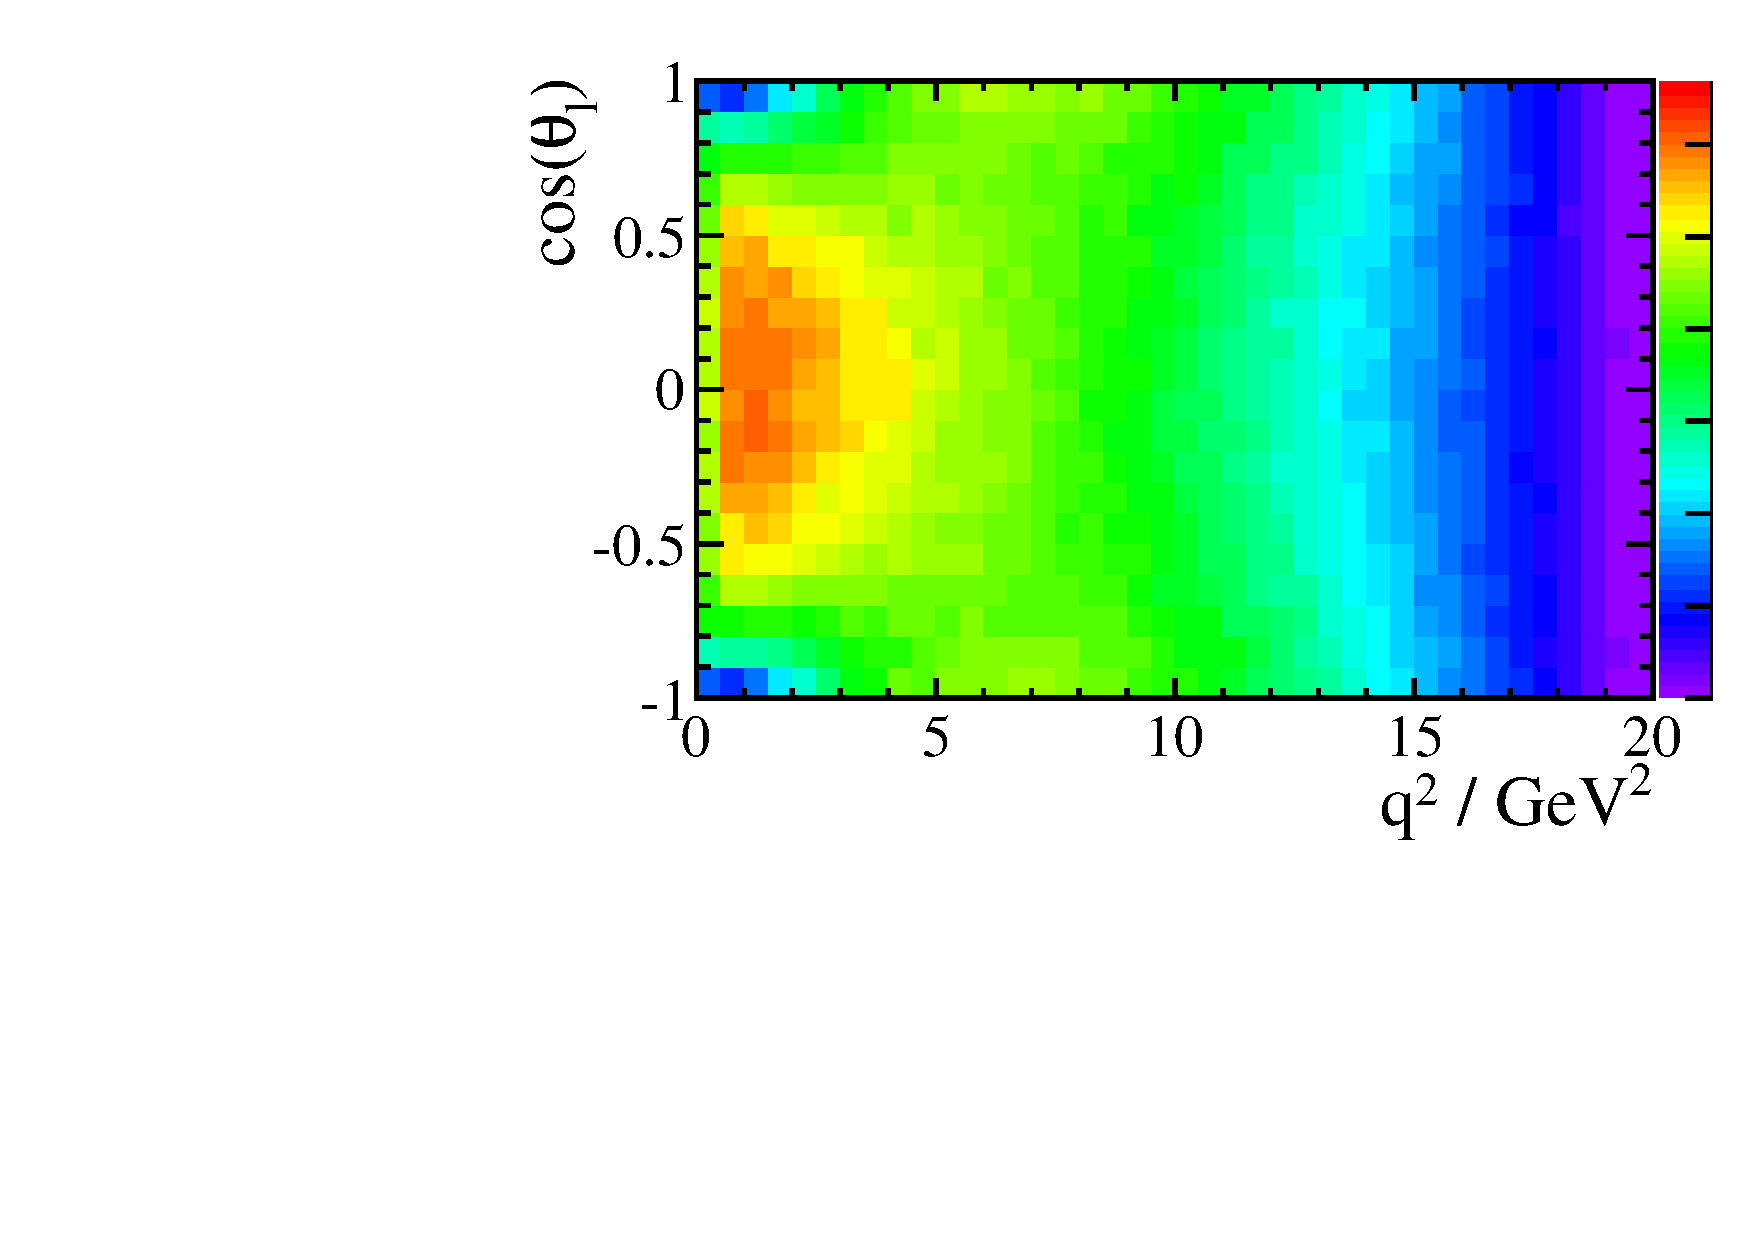
\includegraphics[width=0.48\columnwidth]{chapter5/figs/phsp_ctl_qsq_sel_dist.pdf}}
\subfigure[\ctk v.s. \qsq]{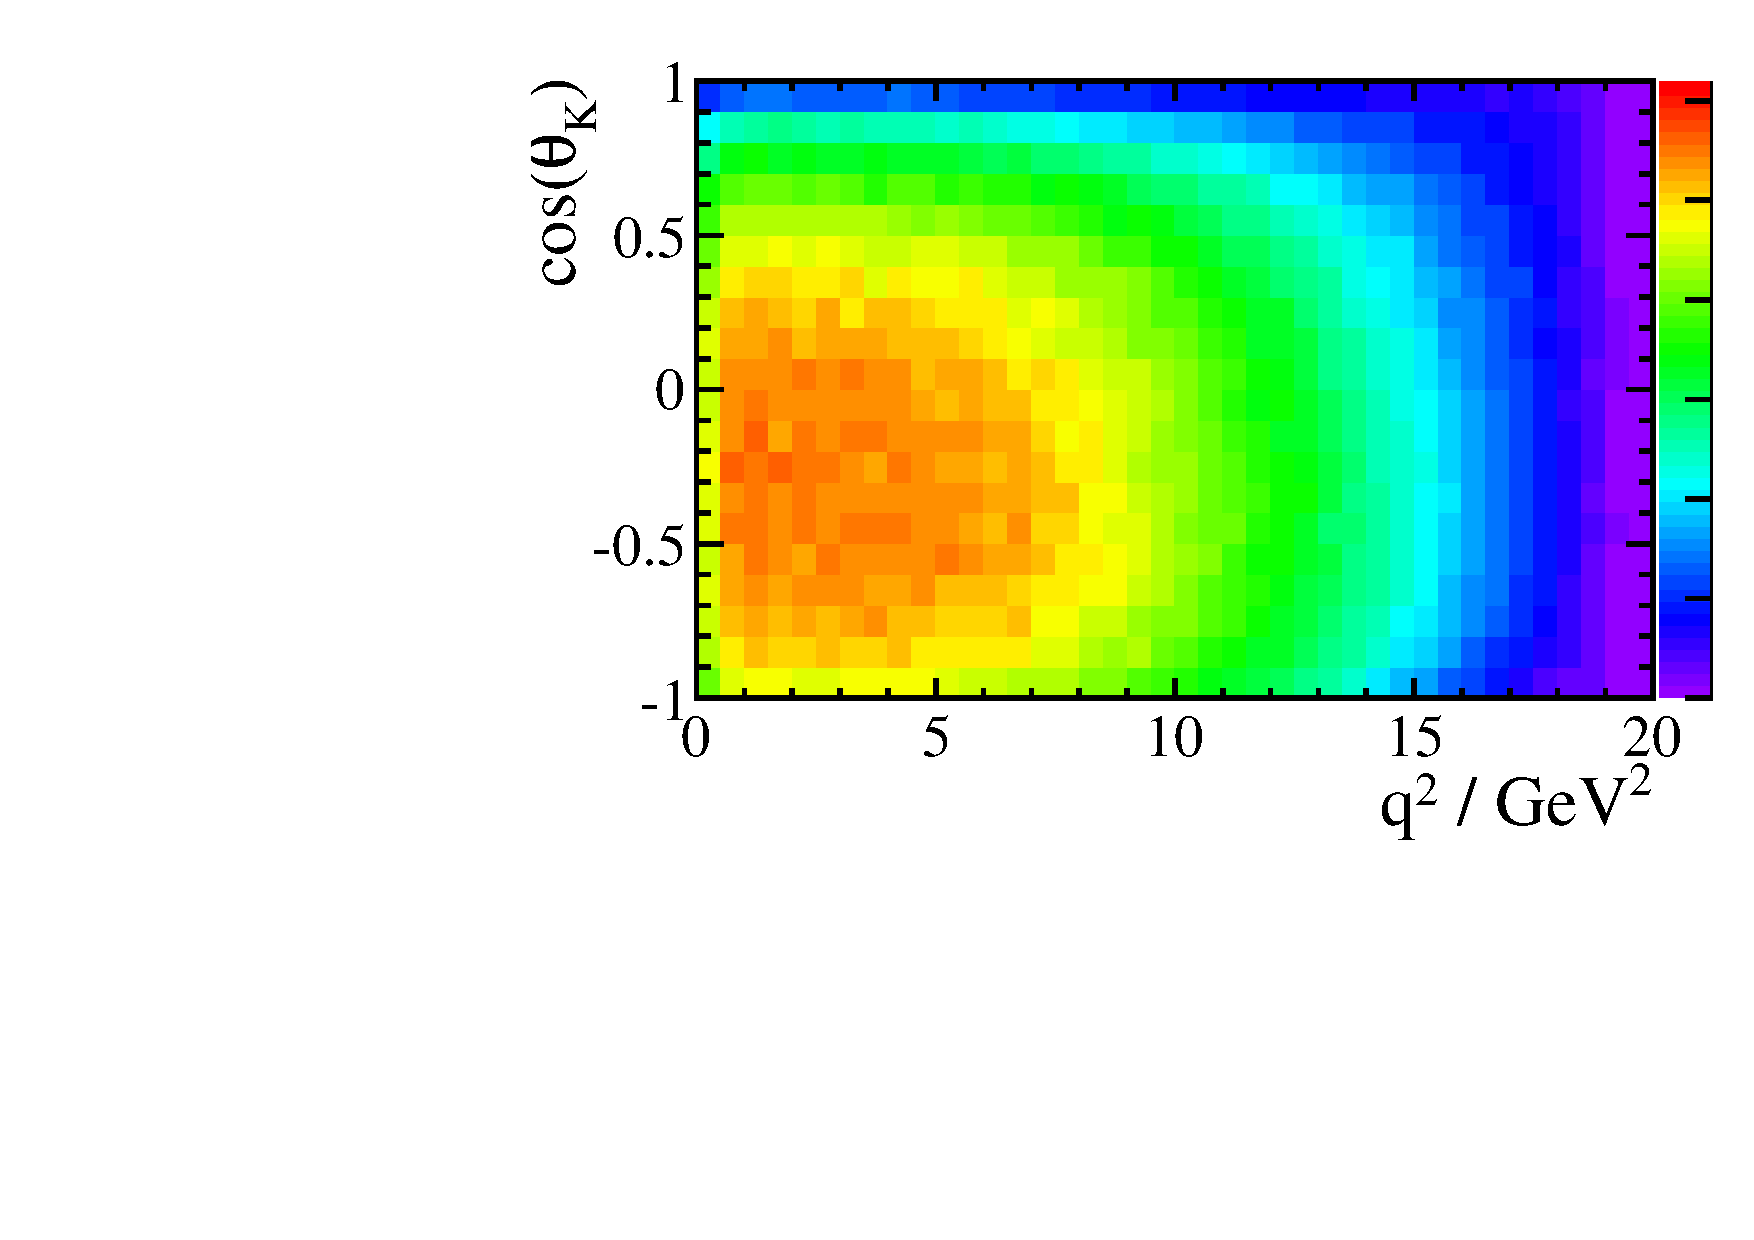
\includegraphics[width=0.48\columnwidth]{chapter5/figs/phsp_ctk_qsq_sel_dist.pdf}}
\subfigure[$\phi$ v.s. \qsq]{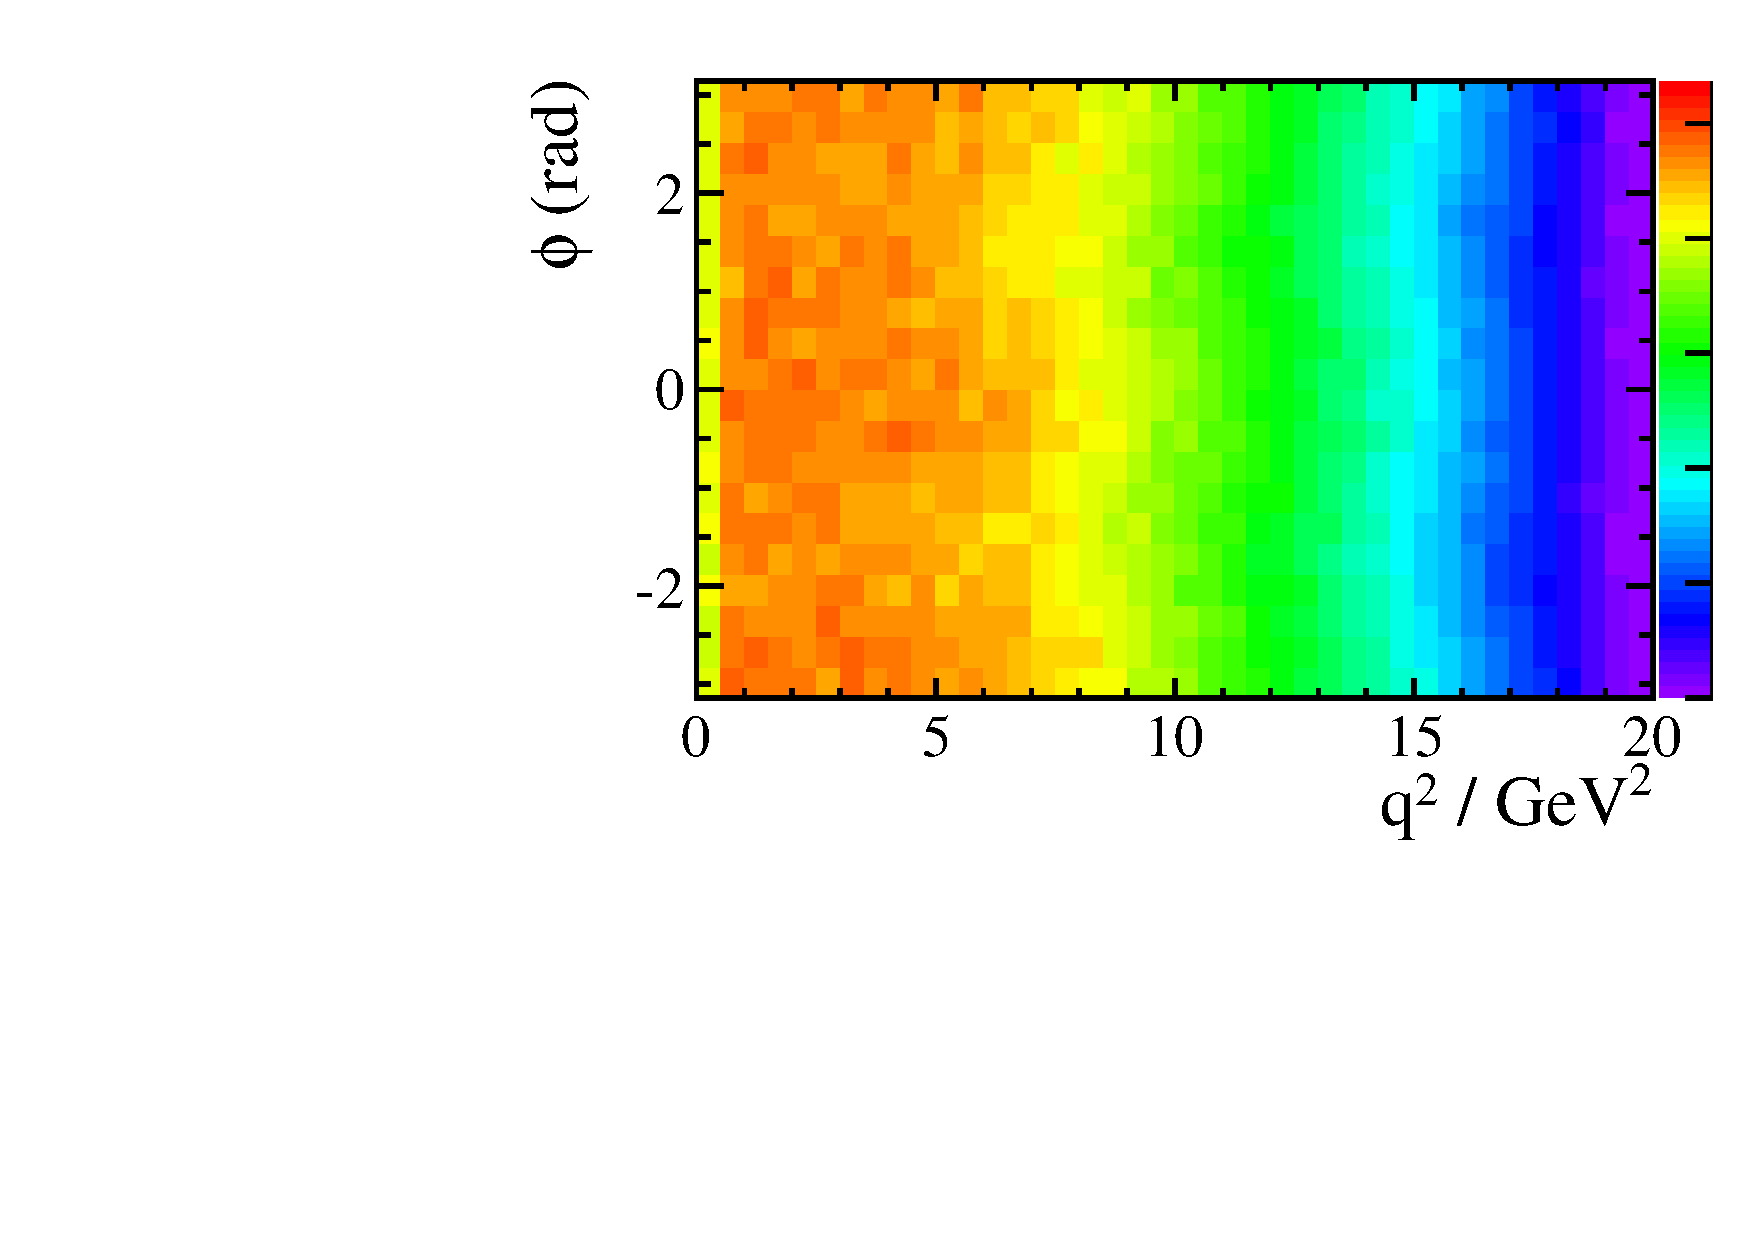
\includegraphics[width=0.48\columnwidth]{chapter5/figs/phsp_phi_qsq_sel_dist.pdf}}
\caption[Two dimensional efficiency for \BdToKstmm simulation.]
{The efficiency for selected phase space simulated \BdToKstmm events. 
In (a), (b), and (c), events are selected in the low \qsq bin ($1 < \qsq < 2 \gevgevcccc$). 
In (d), (e) and (f), the correlation between the individual angles and the full \qsq range is shown.
~\label{fig:phspeff2d} } 
\end{figure}
%It is possible to see the the efficiency is correlated with \qsq but 
%there is no significant correlation between the angles on the level of the binning shown here. 
From this it is possible to see that the efficiency function varies as \qsq, but there is no significant non-factorisable effect in the angles.
This means that the PDFs must be binned in \qsq but can be factorised between the angles.
The efficiency function for a bin in \qsq is given by 
\begin{align}
\epsilon(\ctl, \ctk, \phi, x<\qsq<y)  = \left( \frac{n_{(x<\qsq<y)} }{m_{(x<\qsq<y)} }\right) \times  S_L(\ctl) \times S_K( \ctk ) \times  S_P( \phi ) 
\end{align}
where $S_i$ is the \PDF describing the distribution of offline selected phase 
space events for each angle. 
The generator level \PDF ($G$) is uniform as a function of each of the angles and can be integrated out.

A non-uniform binning scheme was chosen to take advantage of the uneven distribution of the simulated statistics in \qsq. 
At low \qsq, where statistics are higher, bins of 0.1 \gevgevcccc are used. 
Bins of 0.2 \gevgevcccc are used in the \qsq range from 1 to 6 \gevgevcccc, and bins of 0.5 \gevgevcccc above 6 \gevgevcccc 
to the upper limit of 19\gevgevcccc .
These bins are chosen such that there are at least fifteen thousand offline 
selected events in the least populated bin from a total of two million simulated events.

The one-dimensional efficiency is modelled as a 6th order Chebychev polynomial~\cite{CHEBYCHEV}
and normalised such that the polynomial integrates to 1,
\begin{align}
\int S_i(\text{x};p_0,p_1,p_2,p_3,p_4,p_5)\ \deriv\text{x} = 1 \, ,
\end{align}
where $p_i$ are the coefficients of the polynomial. 
In order to acquire higher statistics in each \qsq bin, further reducing the error on the \PDF, 
the efficiency functions for \ctl and $\phi$ are assumed to be symmetric around 0. 
This symmetry holds to the level of CP-violating detector effects which are assumed to be less than 5\%.
The total efficiency is given by
\begin{align}
\epsilon(\qsq,\ctl,\ctk,\phi)_{(x<\qsq<y)} &= \left( \frac{n_{(x<\qsq<y)} }{m_{(x<\qsq<y)} }\right) \nonumber\\
& \times S_L(\ctl;0,a_1,0,a_3,0,a_5) \nonumber\\
& \times  S_K(\ctk;b_0,b_1,b_2,b_3,b_4,b_5) \nonumber\\
& \times S_P(\phi;0,c_1,0,c_3,0,c_5)
\end{align}
where the even (odd) parameters describe the symmetric (anti-symmetric) components of the polynomial.
The efficiency \PDFs for \ctl, \ctk and \varphi for an example low \qsq bin are shown in Fig.~\ref{fig:facpdfs}.
\begin{figure}[tbp]
\centering
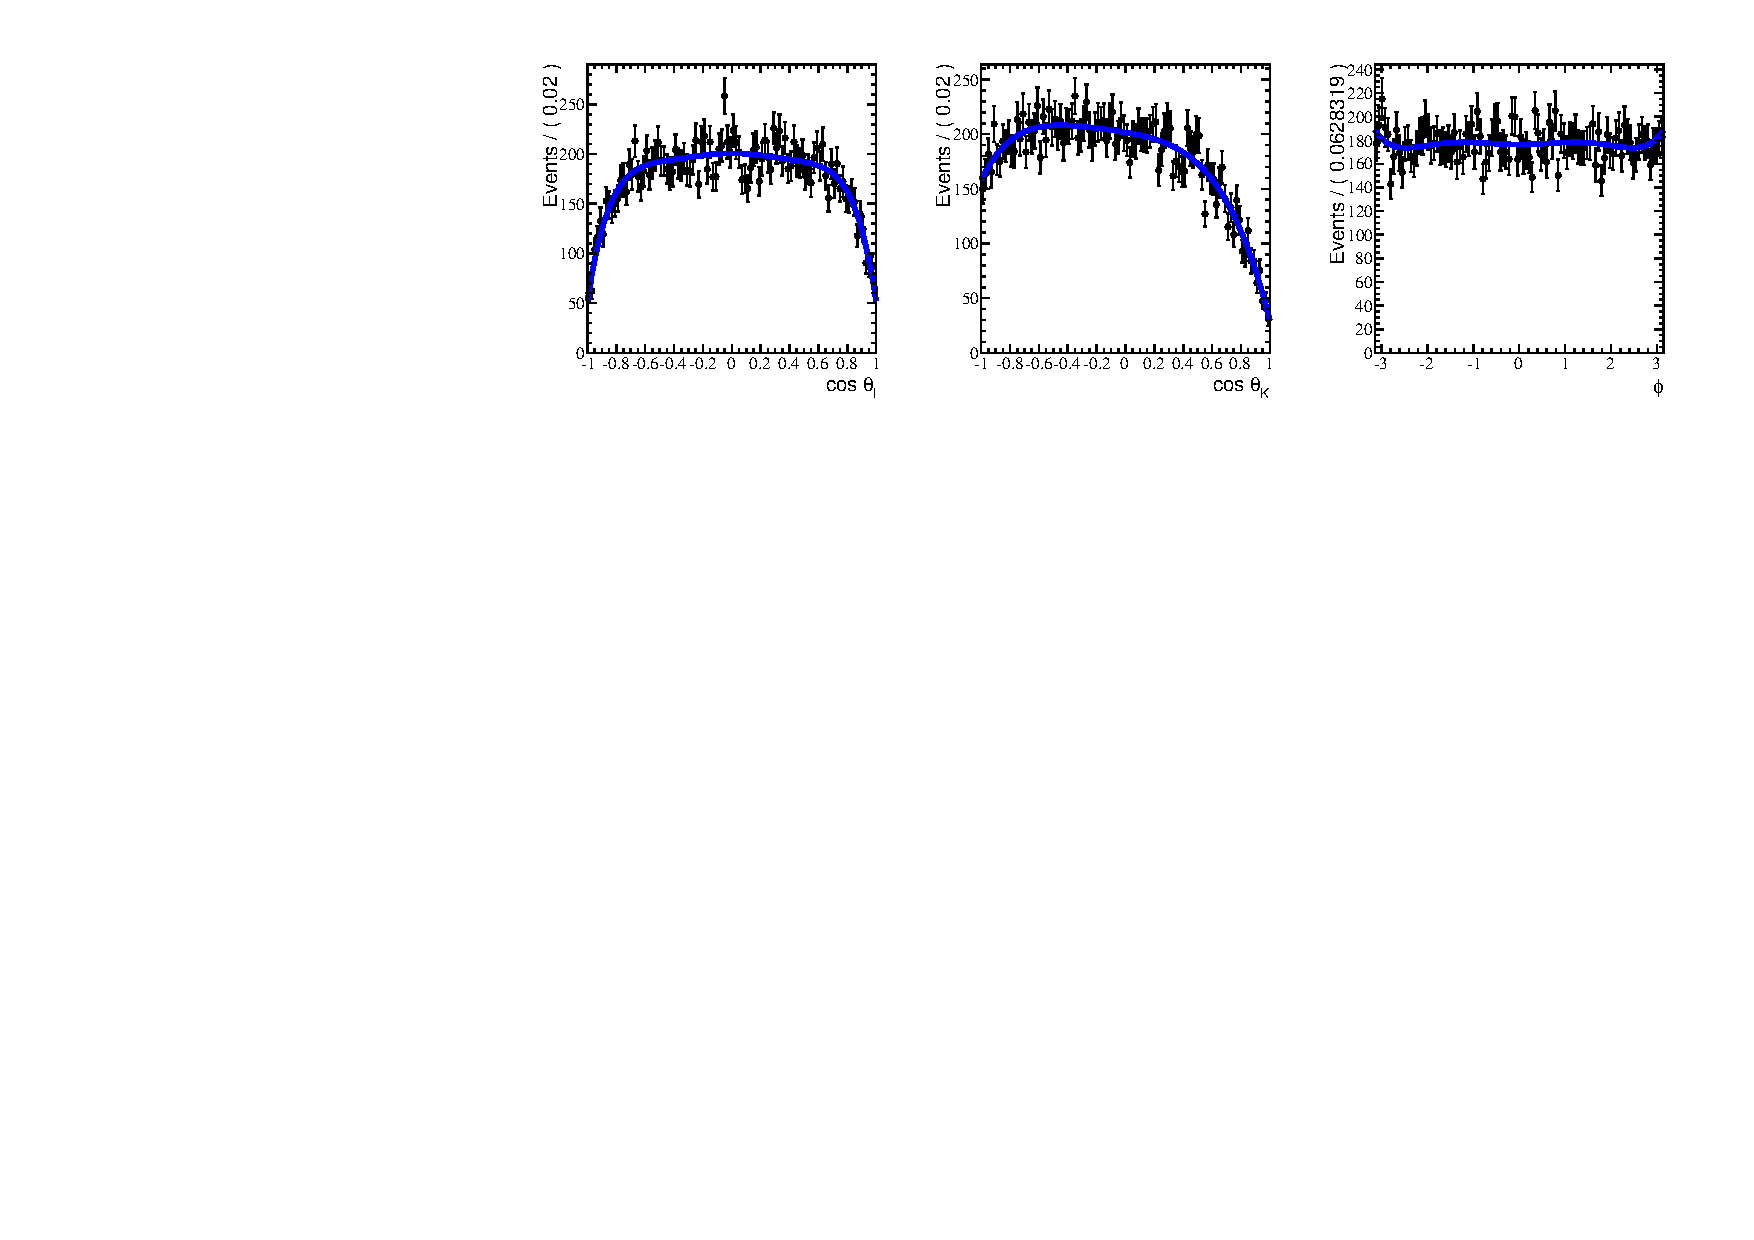
\includegraphics[width=0.96\columnwidth]{chapter5/figs/kstmm_fac_eff_pdfs_nqsqbins.pdf}
\caption[ The simulated \BdToKstmm events and the fitted PDF describing the selected events in \ctl (left), \ctk (middle)
and $\phi$ (right) for the \qsq bin from 0.1 to 0.2 \gevgevcccc.]
{ The angular efficiency in each of the angles for the \qsq bin from 0.1 to 0.2 \gevgevcccc.
The factorised \PDF was fitted to phase space \BdToKstmm simulation. ~\label{fig:facpdfs} }
\end{figure}

The distribution of weights on ten thousand phase space events is given in Fig~\ref{fig:ac2weights}.
\begin{figure}[tbp]
\centering
\subfigure[]{\includegraphics[width=0.48\columnwidth]{chapter5/figs/ac2/phasespace_weight_value.pdf}}
\subfigure[]{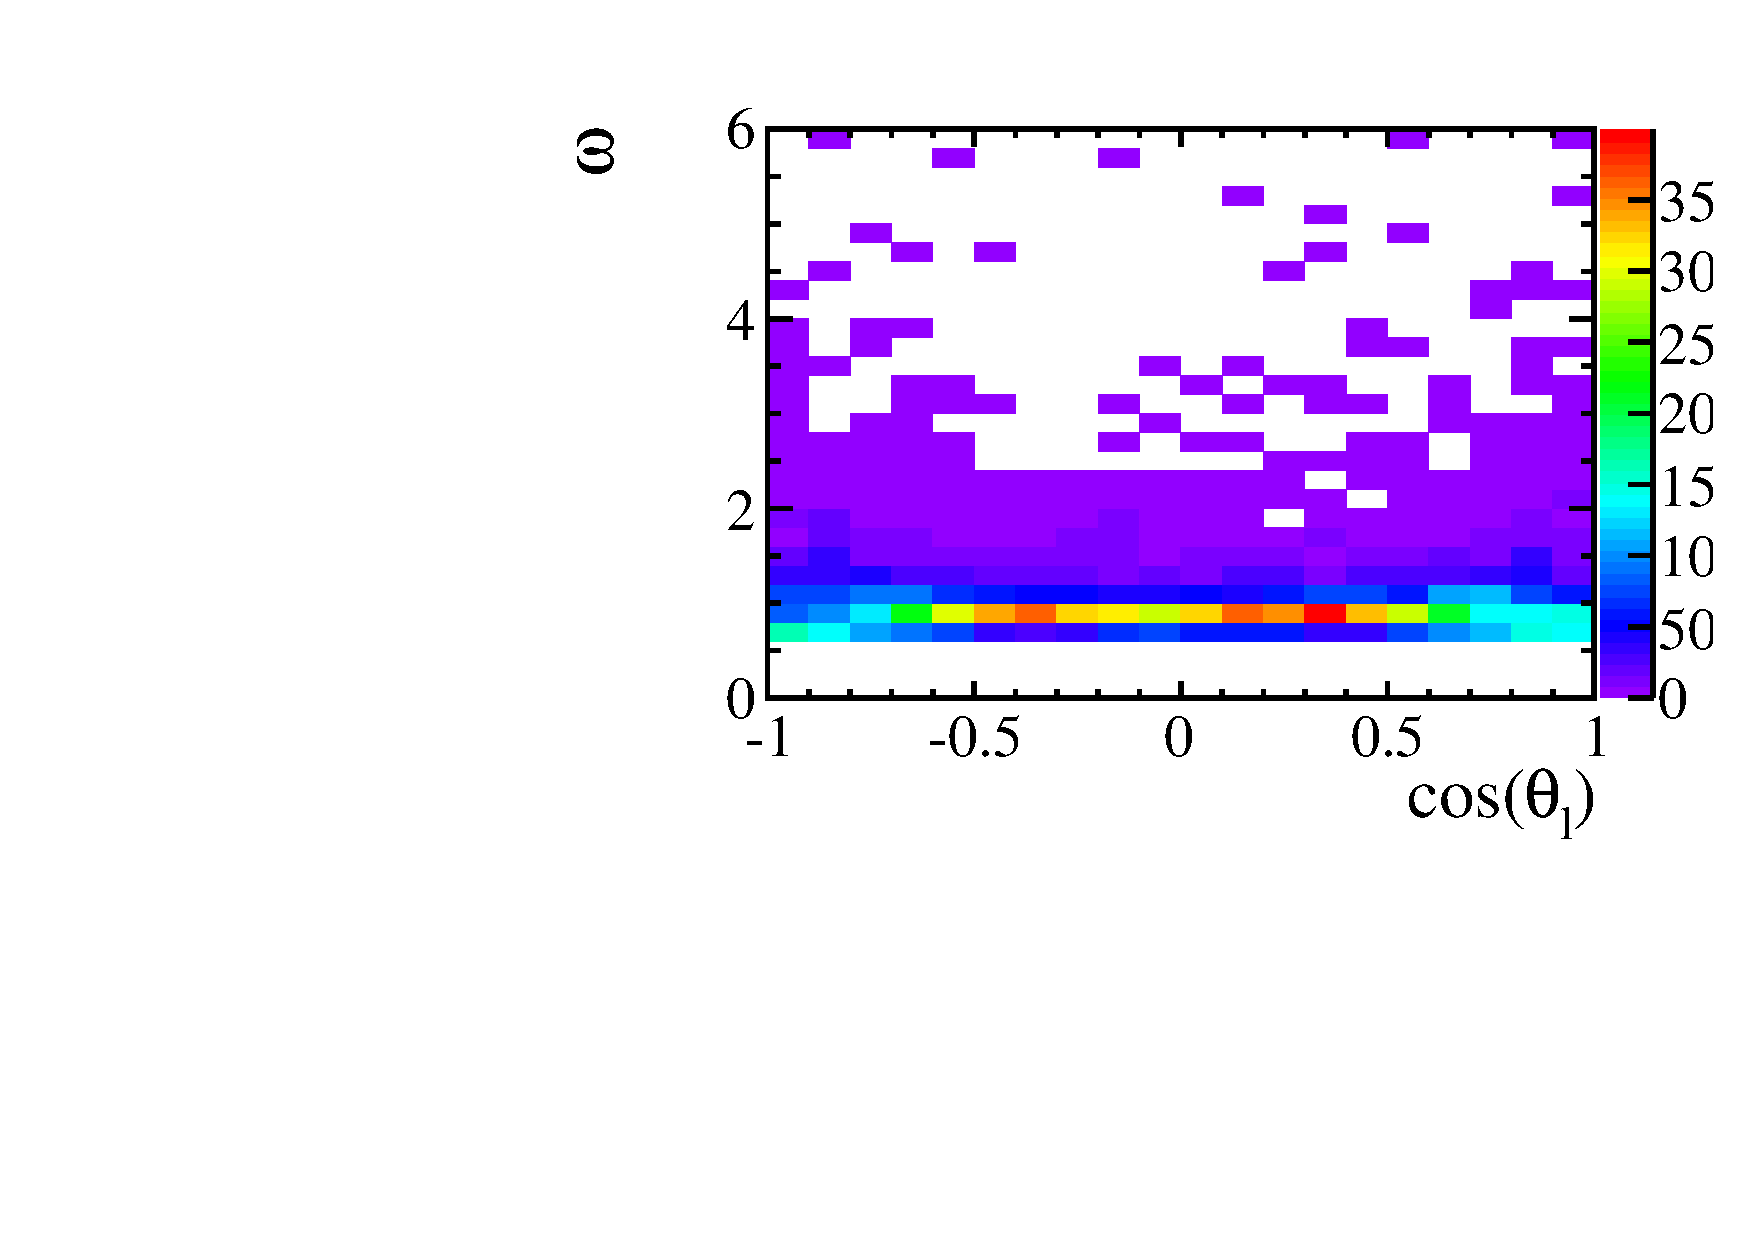
\includegraphics[width=0.48\columnwidth]{chapter5/figs/ac2/phasespace_weight_ctl.pdf}}
\subfigure[]{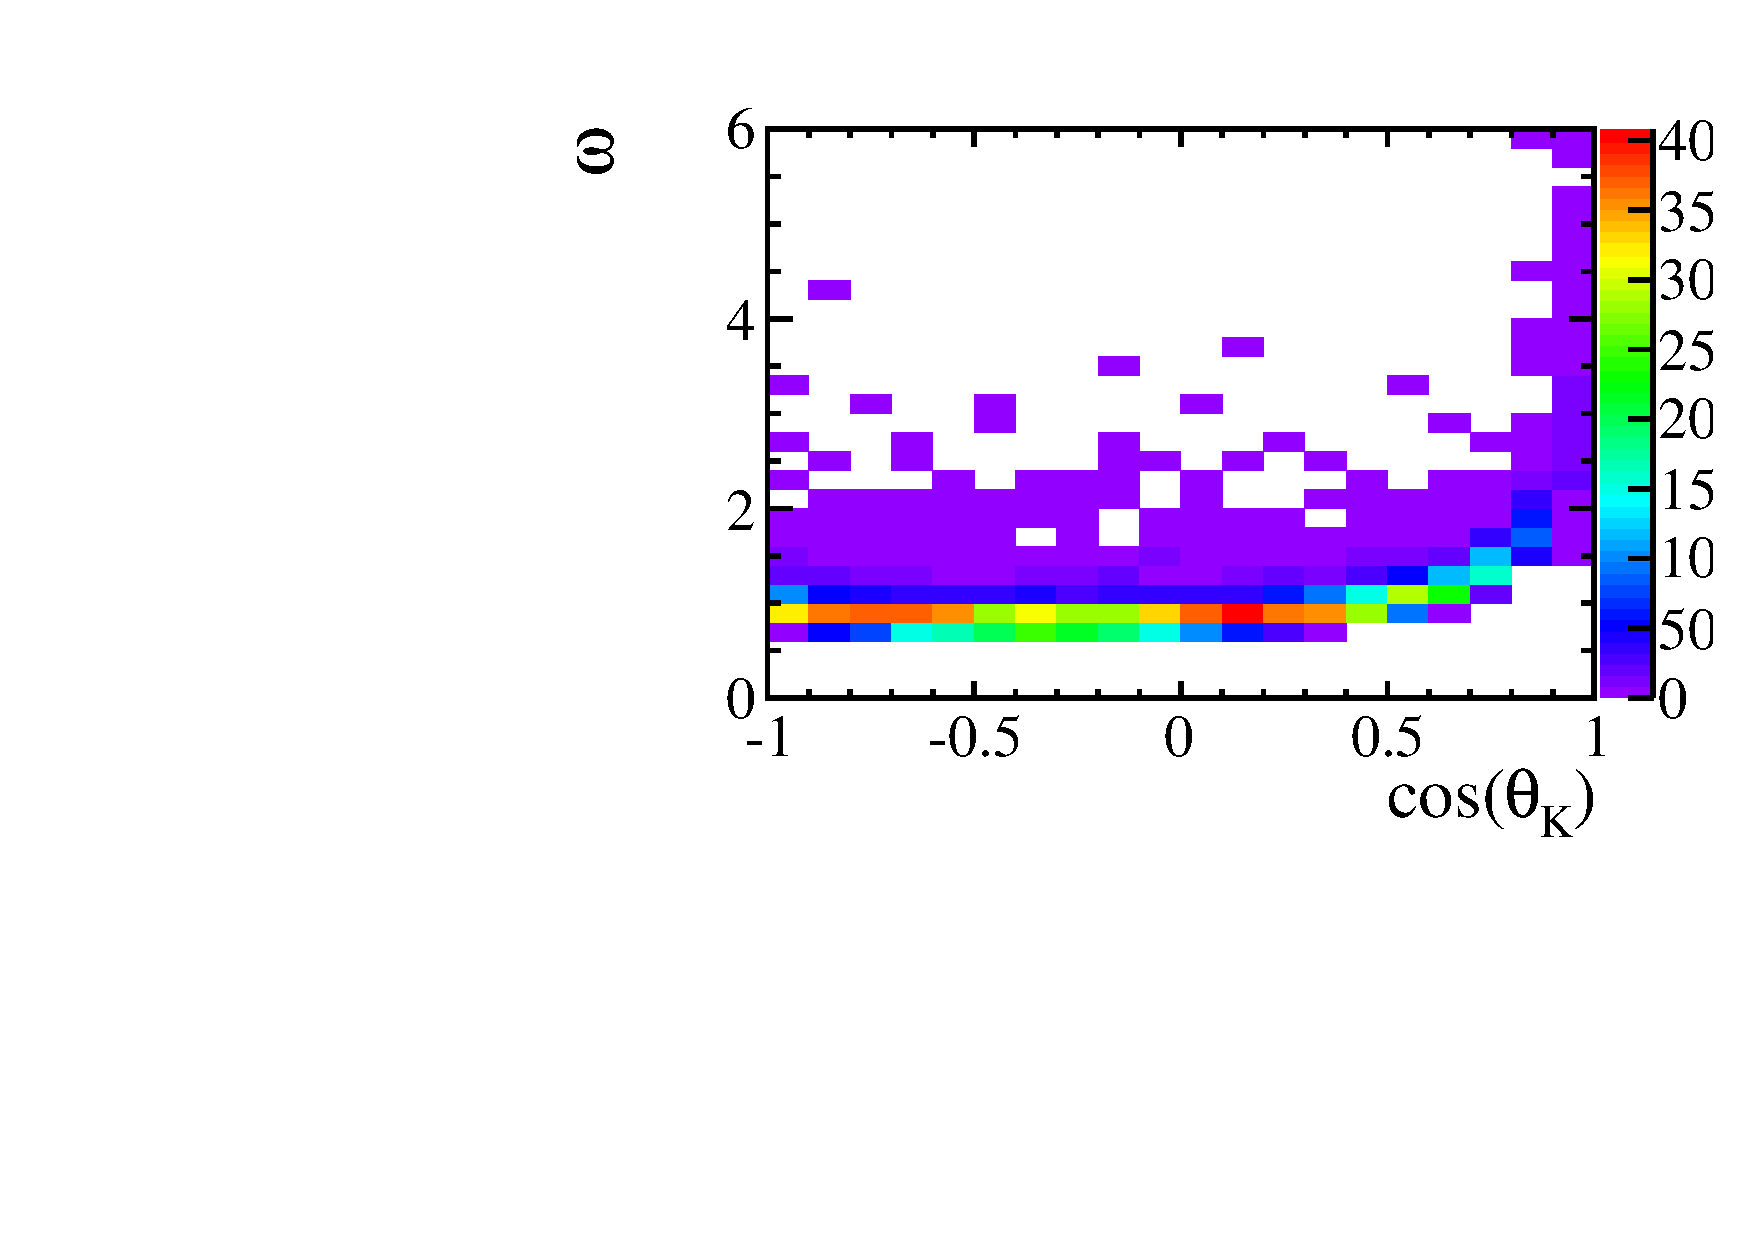
\includegraphics[width=0.48\columnwidth]{chapter5/figs/ac2/phasespace_weight_ctk.pdf}}
%\subfigure[]{\includegraphics[width=0.48\columnwidth]{chapter5/figs/ac2/phasespace_weight_phi.pdf}}
\caption[ The distribution of weights for 10000 phase space simulated \BdToKstmm events.] 
{ The distribution of weights for 10000 phase space simulated \BdToKstmm events and the correlation between 
the weights and \ctl and \ctk. The weights are normalised such that the sum of weights is equal to the 
number of events. The high weights for extreme \ctk and \ctl can be seen. ~\label{fig:ac2weights} }
\end{figure}
The larger weights for extreme \ctl and \ctk regions can be seen.% along with a small variation in \varphi.

\subsubsection{Testing the factorisation}
\label{sec:kstmm:facac:nonfac}

The assumption that the efficiency can be factorised is tested and 
the quality of the fit are assessed by using a variation of the binned $\chi^2$ test.
This modified test compares the distribution of data events used to fit a \PDF to the 
distribution of toy Monte Carlo events generated from the fitted \PDF.
The number of toy Monte Carlo events generated from the fitted \PDF 
using an accept/reject method was scaled to one hundred times the number of data events.
The phase space of \ctl, \ctk and $\phi$ was divided up into one thousand bins.
The pull value for each bin is calculated from
\begin{align}
p^i = n^{i}_{Data} - \left(\frac{n_{Data}^i - 10^{-2} n^{i}_{MC} }{ \sigma }\right)
\end{align}
where the error is defined as
\begin{align}
\sigma = \sqrt{( n_{Data}^i + 10^{-2} n_{MC} )} \, .
\end{align}
If the \PDF is a good fit to the data then the pull values should be normally distributed.
Here the `data' is the offline selected sample of phase space \BdToKstmm simulated events. 
Pull distributions for one low and one high \qsq bin are shown in Fig.~\ref{fig:facpulldist}.
\begin{figure}[tbp]
\centering
\subfigure[]{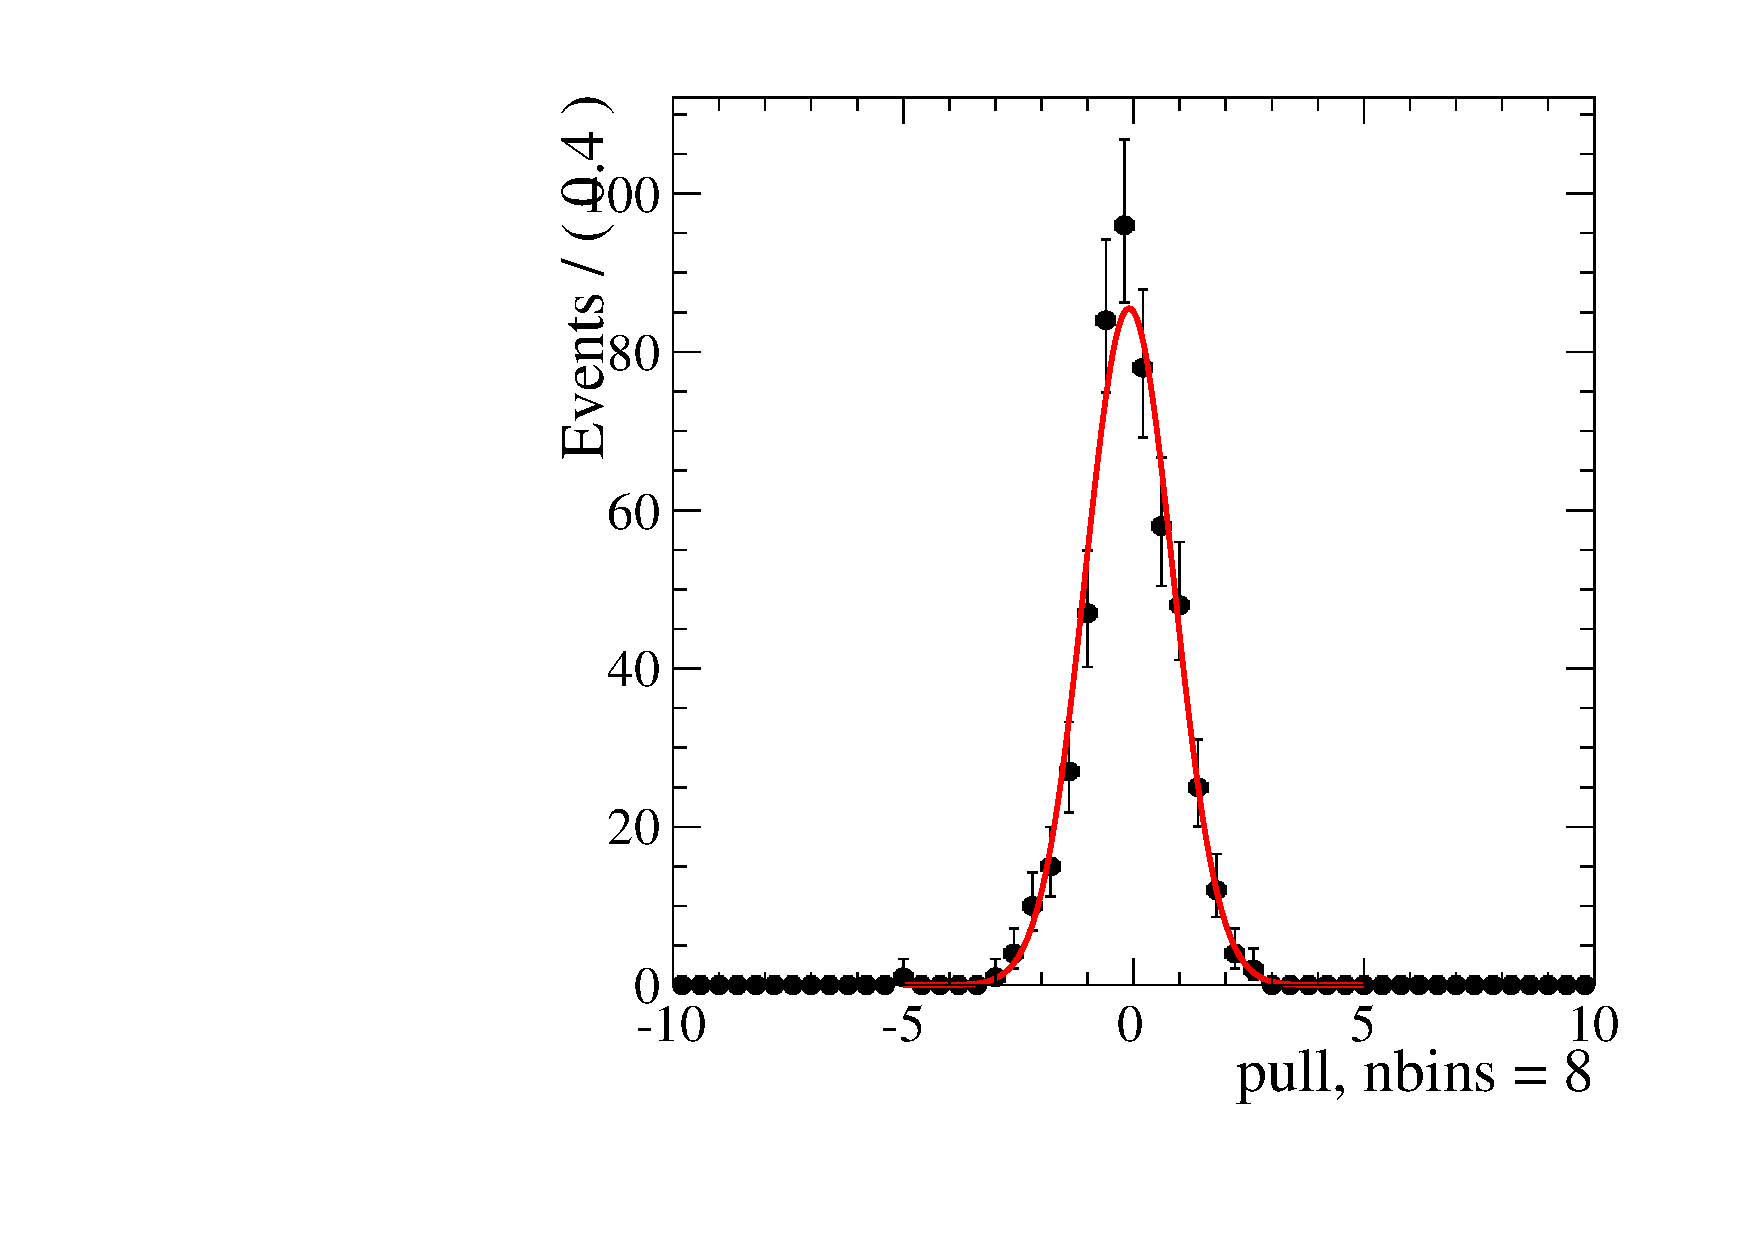
\includegraphics[width=0.48\columnwidth,page=1]{chapter5/figs/pull_dist_qsq_bins.pdf}}
\subfigure[]{\includegraphics[width=0.48\columnwidth,page=50]{chapter5/figs/pull_dist_qsq_bins.pdf}}
\caption [ The pull distribution of a toy simulation from the factorised \PDFs.] 
{ The pull distribution of a toy simulation from the factorised \PDFs.
A low \qsq bin (a) ($1<\qsq<2\gevgevcccc$) and a high \qsq bin (b) ($15<\qsq<15.5\gevgevcccc$). 
The fit for both distributions is compatible with a Gaussian of zero mean and unit width. ~\label{fig:facpulldist} }
\end{figure}
Both pull distributions are compatible with a Gaussian with zero mean and unit width.
The mean and width of the pull distribution for each bin in \qsq are given in Fig.~\ref{fig:facpulldistall}.
\begin{figure}[tbp]
\centering
\subfigure[]{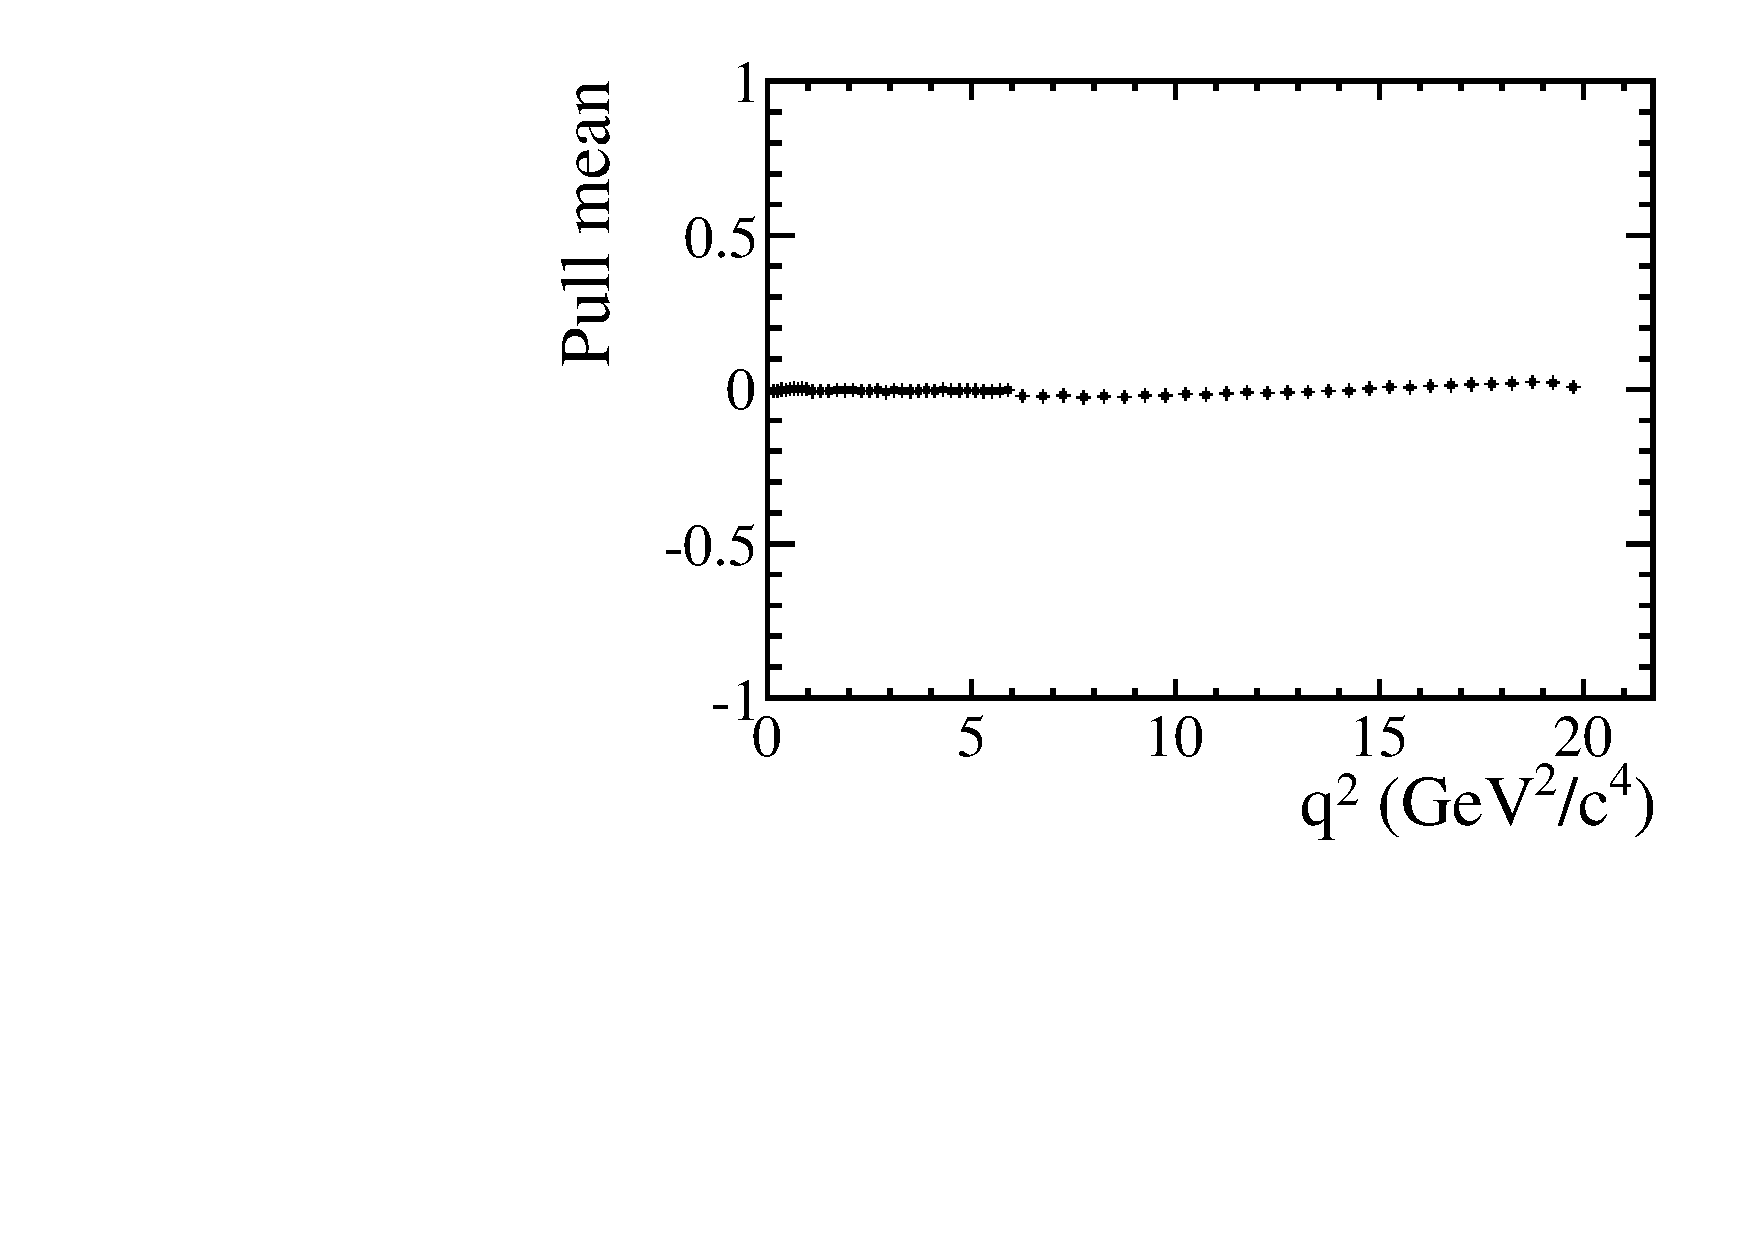
\includegraphics[width=0.48\columnwidth]{chapter5/figs/ac2/fiteff_results_62_pull_meangraph.pdf}}
\subfigure[]{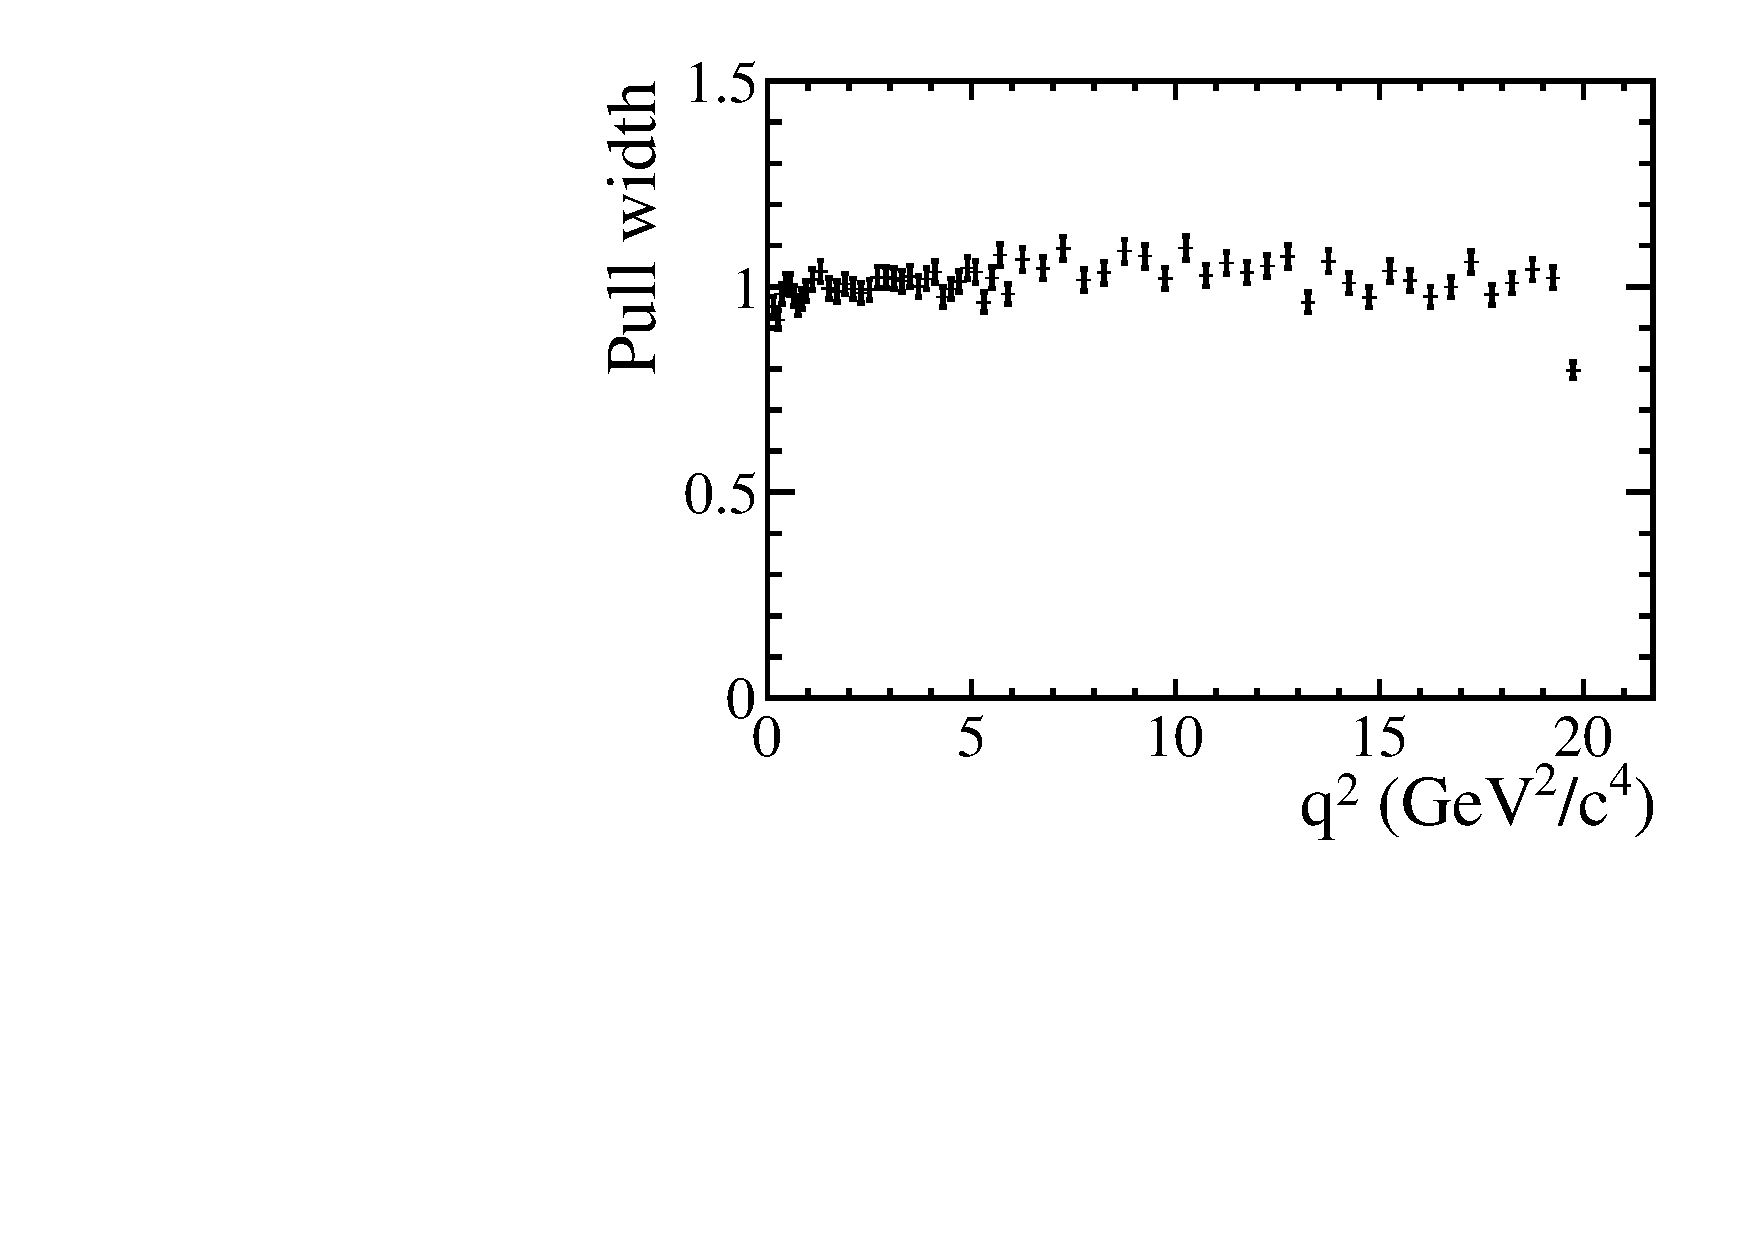
\includegraphics[width=0.48\columnwidth]{chapter5/figs/ac2/fiteff_results_62_pull_pullgraph_new.pdf}}
\caption [ The pull distribution of a toy simulation from the factorised \PDFs.] 
{ The (a) mean and (b) width of each pull distribution of a toy simulation from the factorised \PDFs in bins of \qsq.
The bins are all compatible with a Gaussian of zero mean and unit width. ~\label{fig:facpulldistall} }
\end{figure}
This shows that there are no regions of great discrepancy between the simulation and the factorised \PDF in these bins of \qsq.

The factorisation of the efficiency allows for a more precise acceptance correction at the cost of incurring a 
possible source of systematic uncertainty associated with integrating over non-factorisable effects.
The factorisation was also tested by comparing the re-weighted phase space simulated events to the 
generator level distributions in each of the factorised dimensions.

%The degree to which non-factorisable effects can be ignored is tested by
%multiplying the efficiency function with a non-factorisable function,
%\begin{align}
%f(\ctl,\ctk) = 1 + \alpha\sin(\pi\ctl)\sin(\pi\ctk)
%\end{align}
%where $\alpha$ is a scaling factor. The efficiency function is modelled as
%\begin{align}
%\epsilon^{'}(\qsq,\ctl,\ctk,\phi)_{(x<\qsq<y)} = \epsilon(\qsq,\ctl,\ctk,\phi)_{(x<\qsq<y)} \times f(\ctl,\ctk) \, .
%\end{align}
%The mean and width of a Gaussian fit to the pull distributions for various values of $\alpha$
%are shown in Fig.~\ref{fig:nonfactest}.
%\begin{figure}[tbp]
%\centering
%\dots
%\caption{ The pull mean and pull width for a Gaussian fit to the pull distribution between simulation and 
%toy Monte Carlo generated from the fitted efficiency as a function of the non-factorisable 
%scaling factor, $\alpha$. ~\label{fig:nonfactest} }
%\end{figure}

\subsection{Re-weighted phase space distributions}

The most basic test of an acceptance correction is that the original generator 
level distribution used to create the acceptance correction can be recovered.
In this case the phase space distribution %given in Fig.~\ref{fig:phsp}
should be recovered when the phase space candidates are themselves weighted.
The number of re-weighted \BdToKstmm candidates per bin in phase space is given by 
\begin{align}
N_{\text{bin}} = \sum_{i=1}^{ncand} \frac{1}{\epsilon(\ctl,\ctk,\phi)_i} = \sum_{i=1}^{ncand} \omega_i .
\end{align}
which can be compared to the expected number of generator level events in that bin. 

The weighted distributions for the $k$-nearest-neighbour acceptance correction method are shown in
Fig.~\ref{fig:corrphsp1}.
\begin{figure}[tbp]
\centering
\subfigure[]{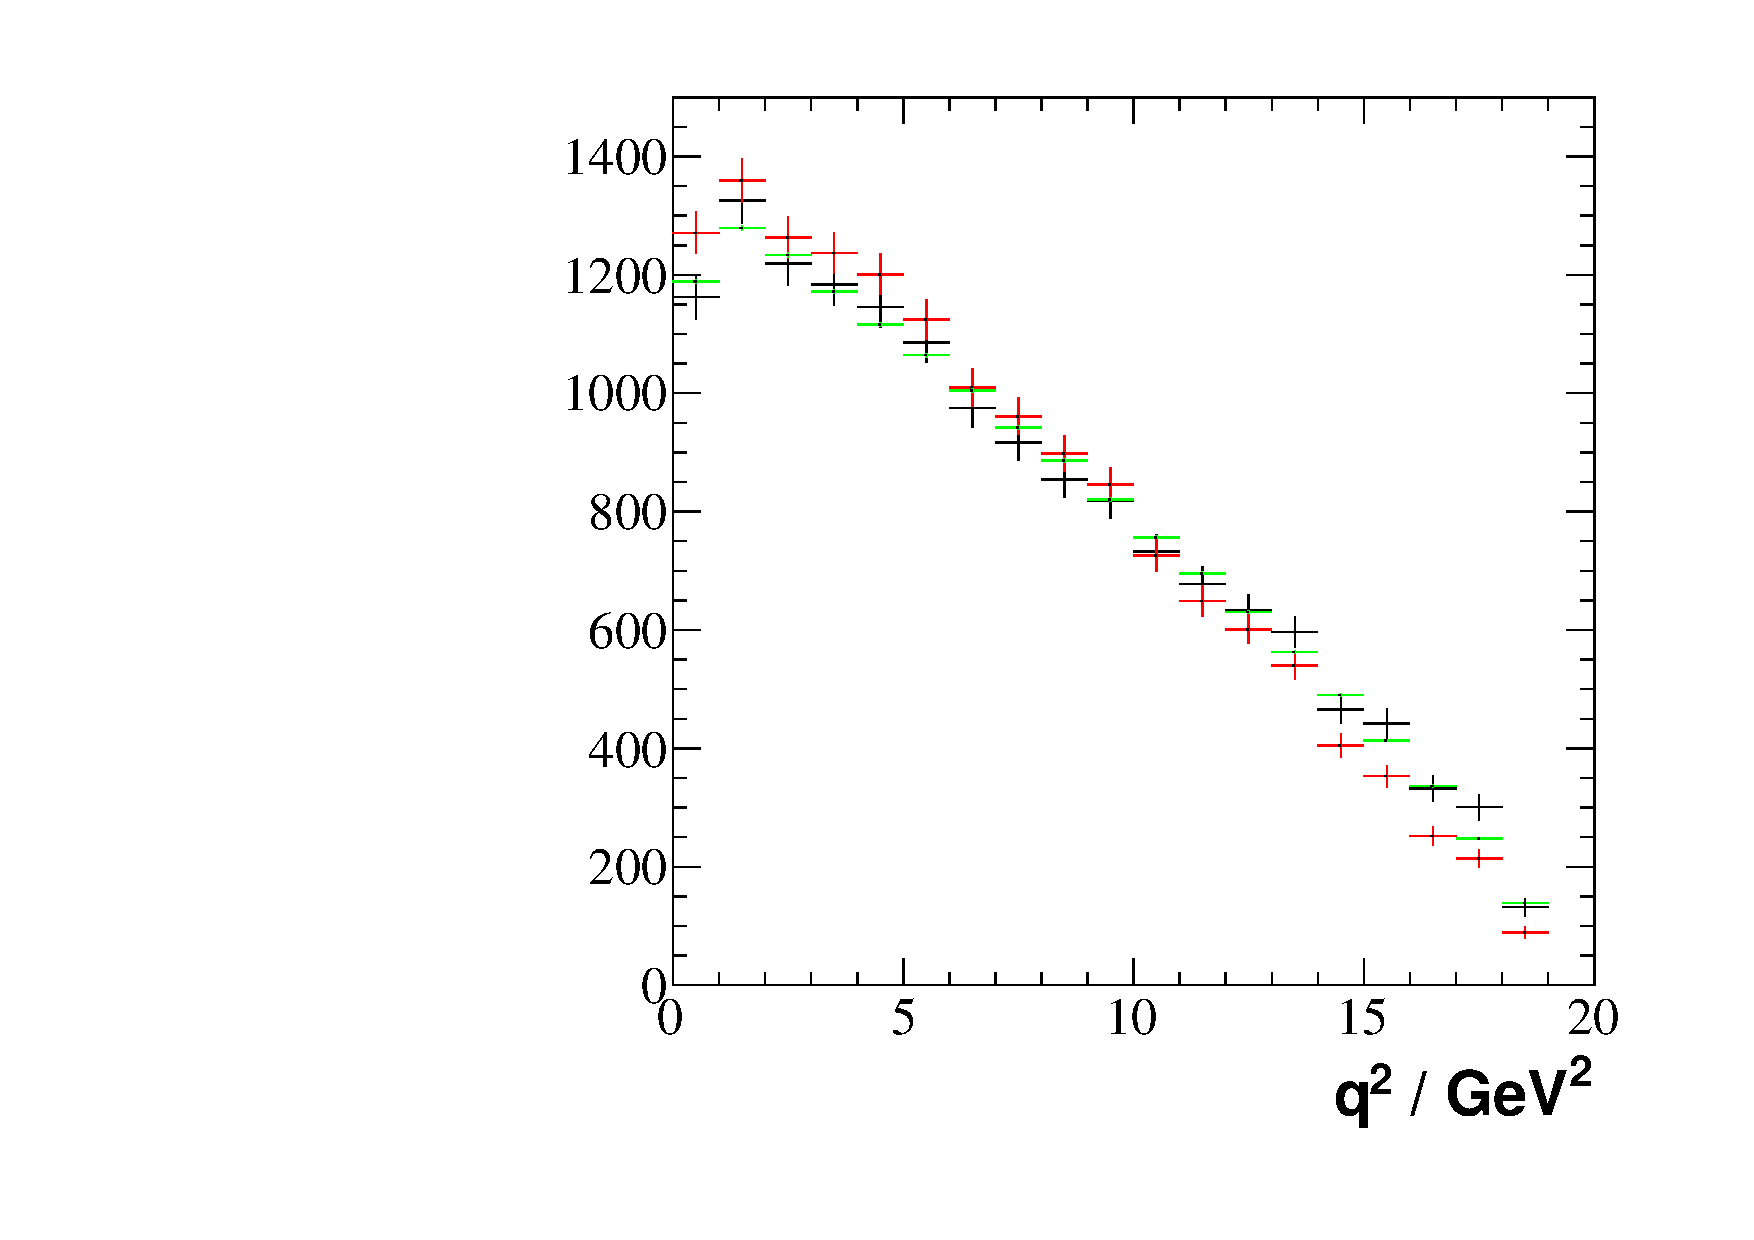
\includegraphics[width=0.32\columnwidth]{chapter5/figs/ac1/CorrectionsWithGen_Qsquare.pdf}}
\subfigure[]{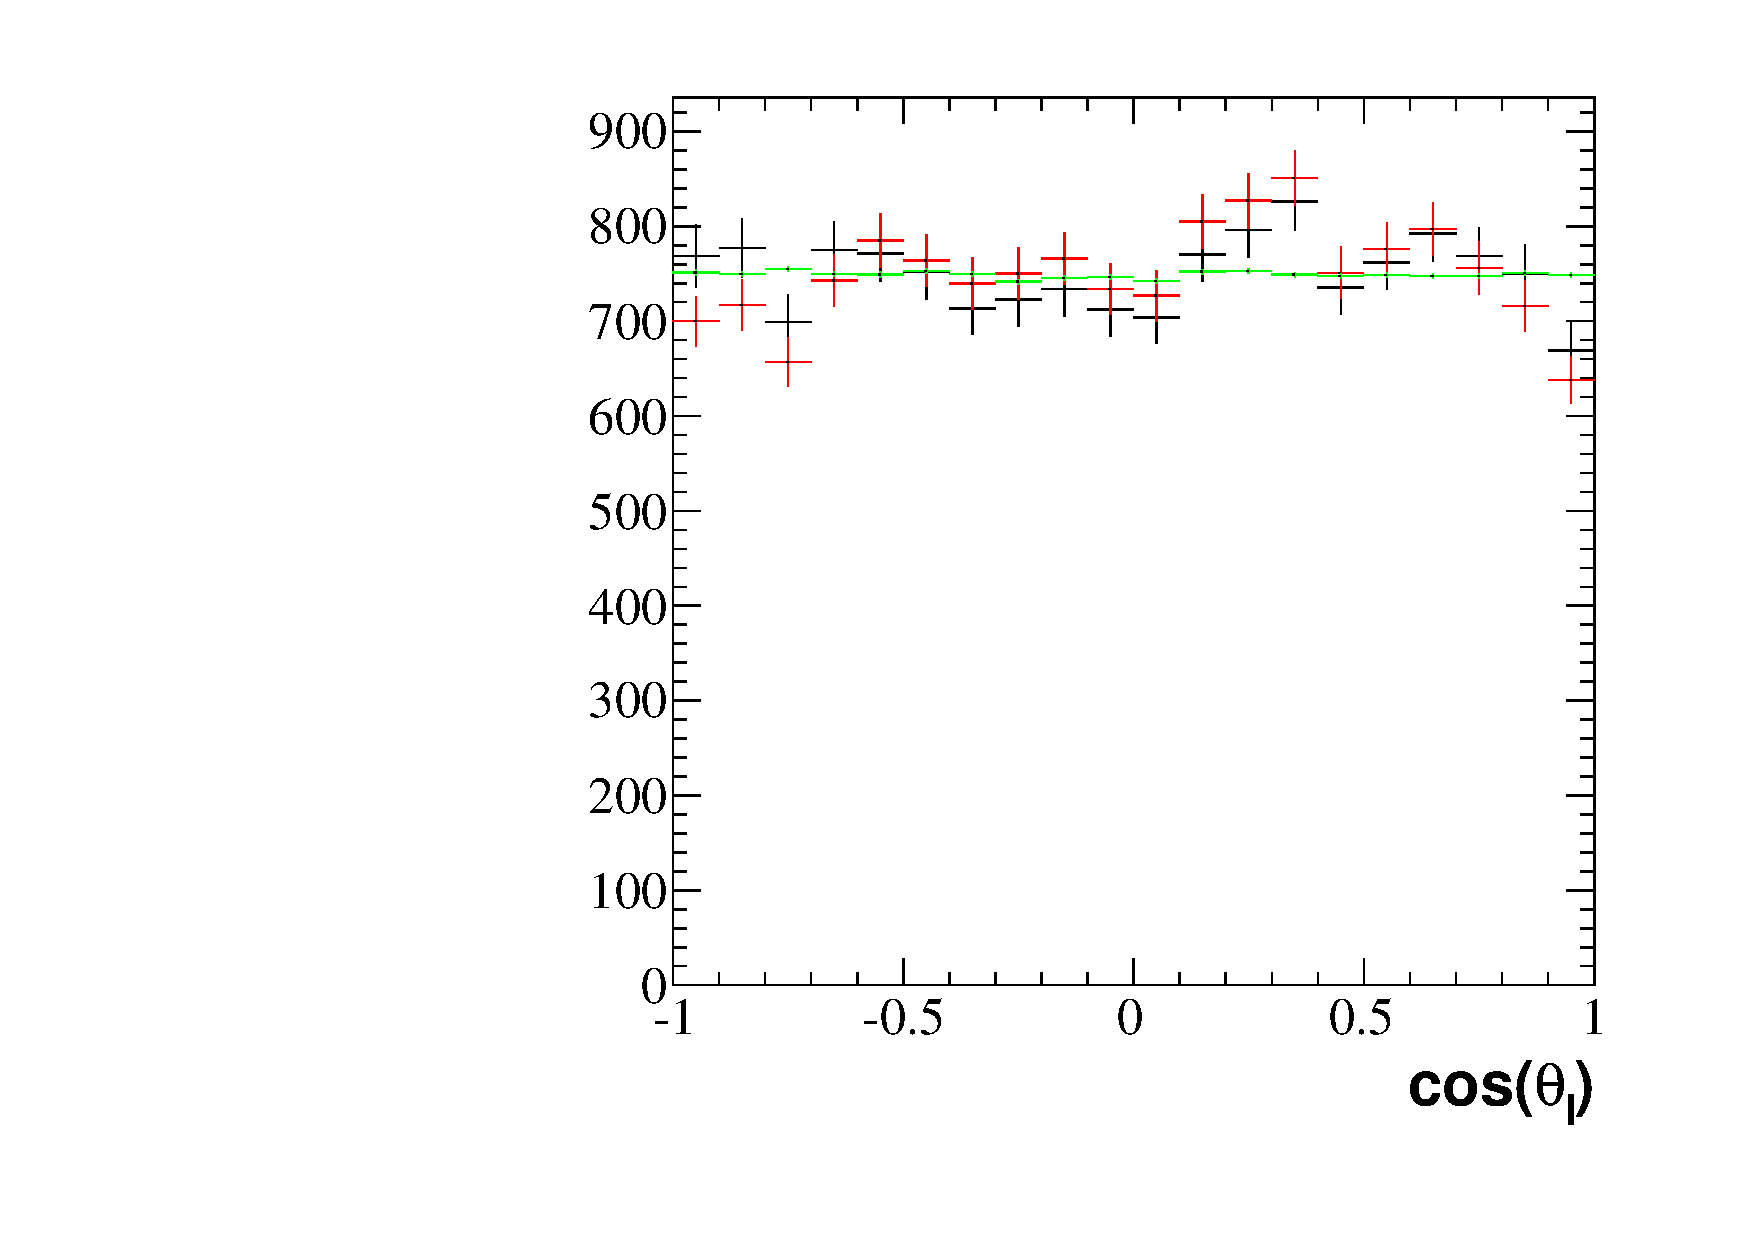
\includegraphics[width=0.32\columnwidth]{chapter5/figs/ac1/CorrectionsWithGen_ThetaL.pdf}}
\subfigure[]{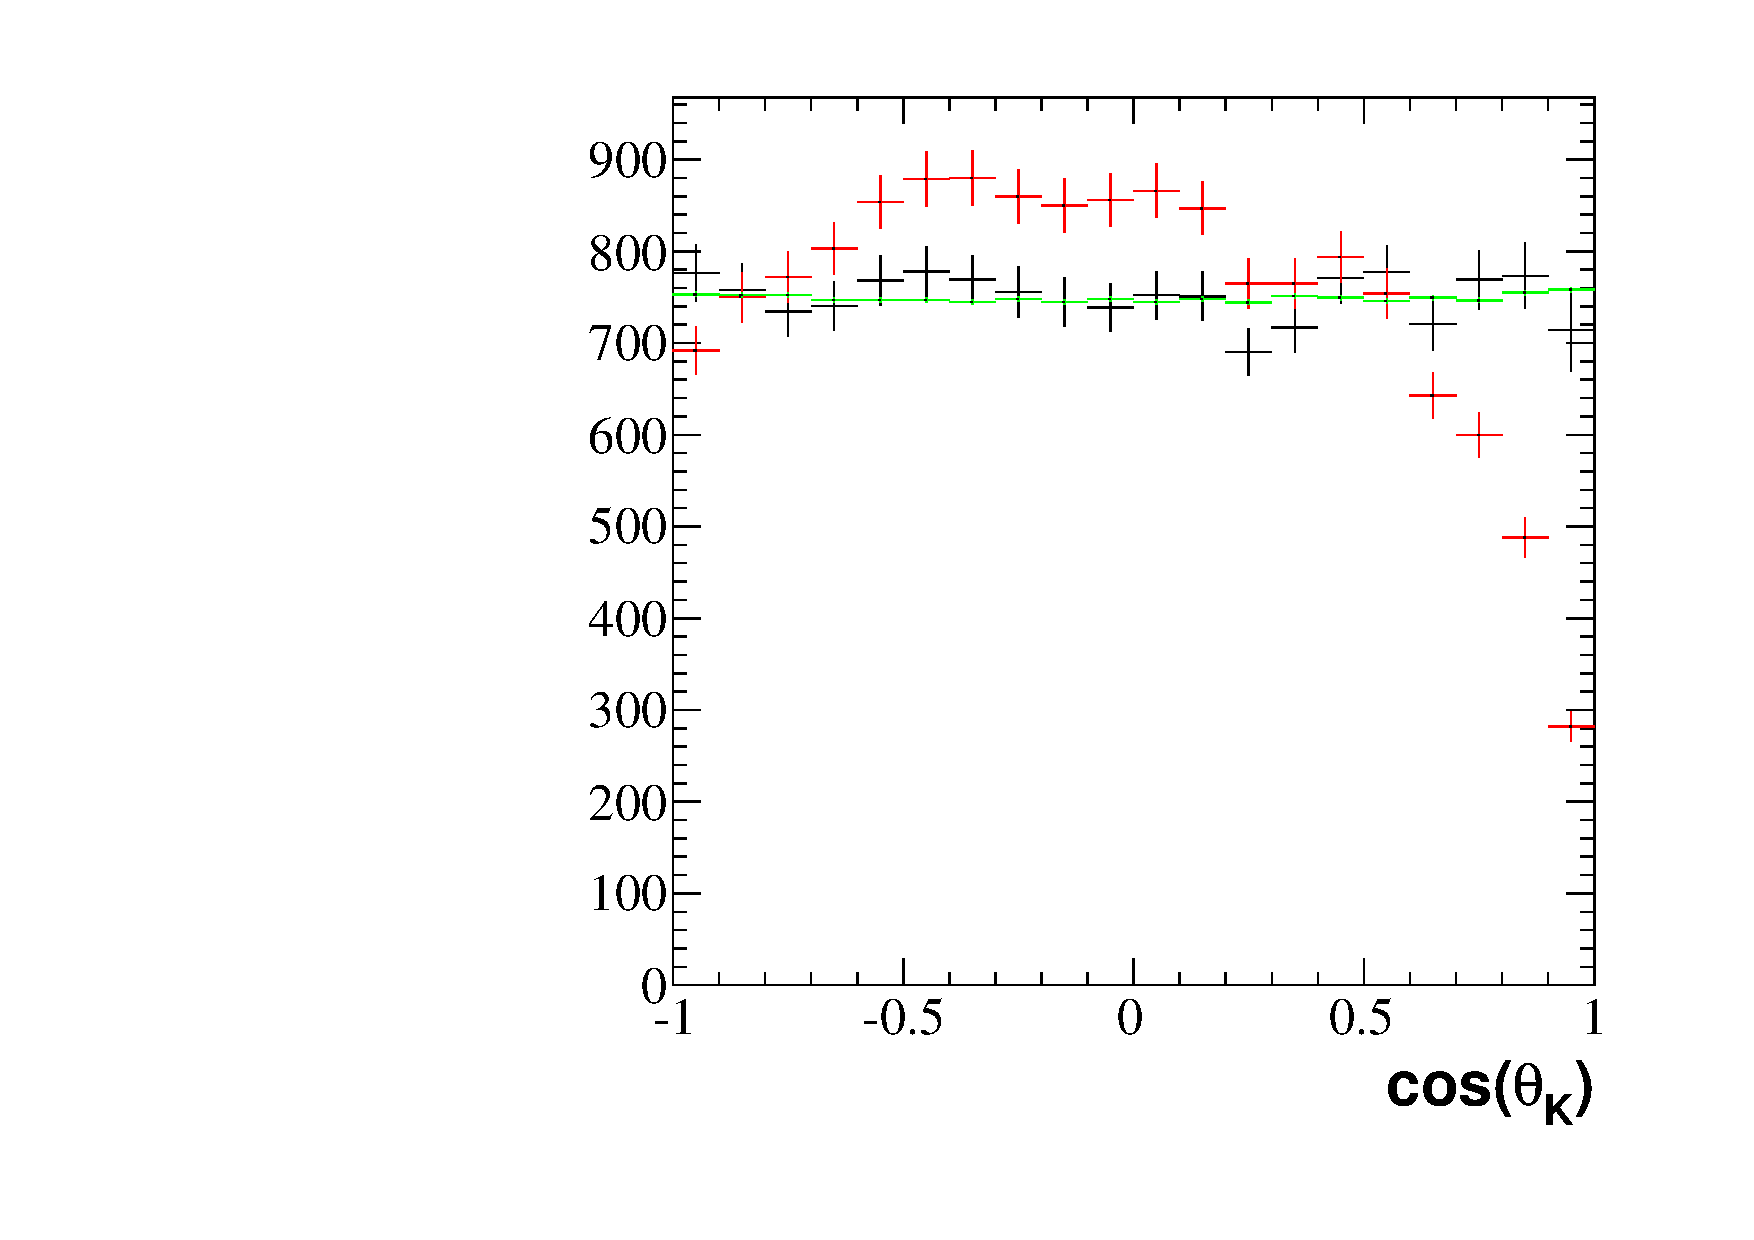
\includegraphics[width=0.32\columnwidth]{chapter5/figs/ac1/CorrectionsWithGen_ThetaK.pdf}}
\caption{Generated (green), offline selected (red) and re-weighted (black) events for  \BdToKstmm using the 
$k$-nearest-neighbour acceptance correction method.~\label{fig:corrphsp1}}
\end{figure}
Is it possible to see that the efficiency at extreme \ctk and extreme \ctl is recovered. 

The weighted distributions for the factorised acceptance correction method are shown in Fig.~\ref{fig:corrphsp2}.
\begin{figure}[tbp]
\centering
\subfigure[]{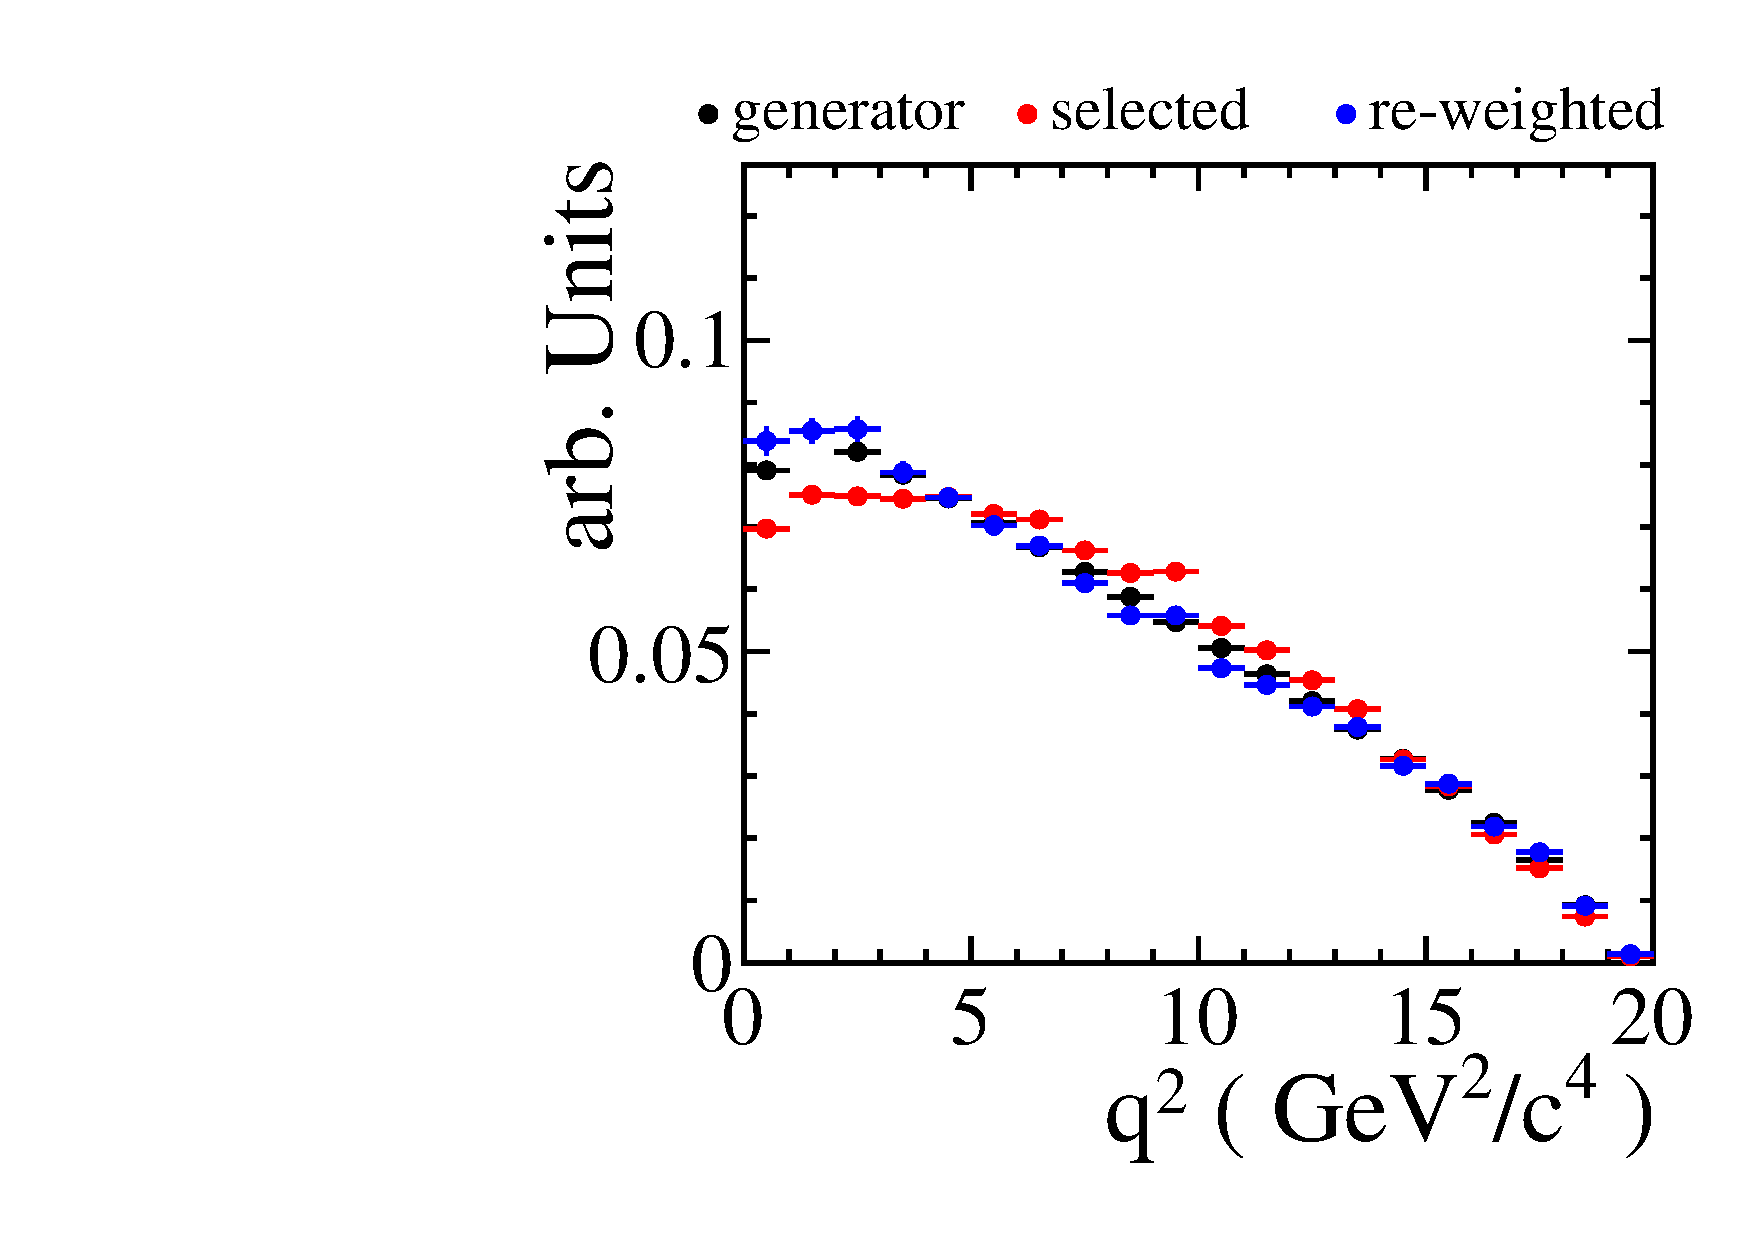
\includegraphics[width=0.48\columnwidth]{chapter5/figs/ac2/CorrectionsWithGen_Qsquare_new.pdf}}
\subfigure[]{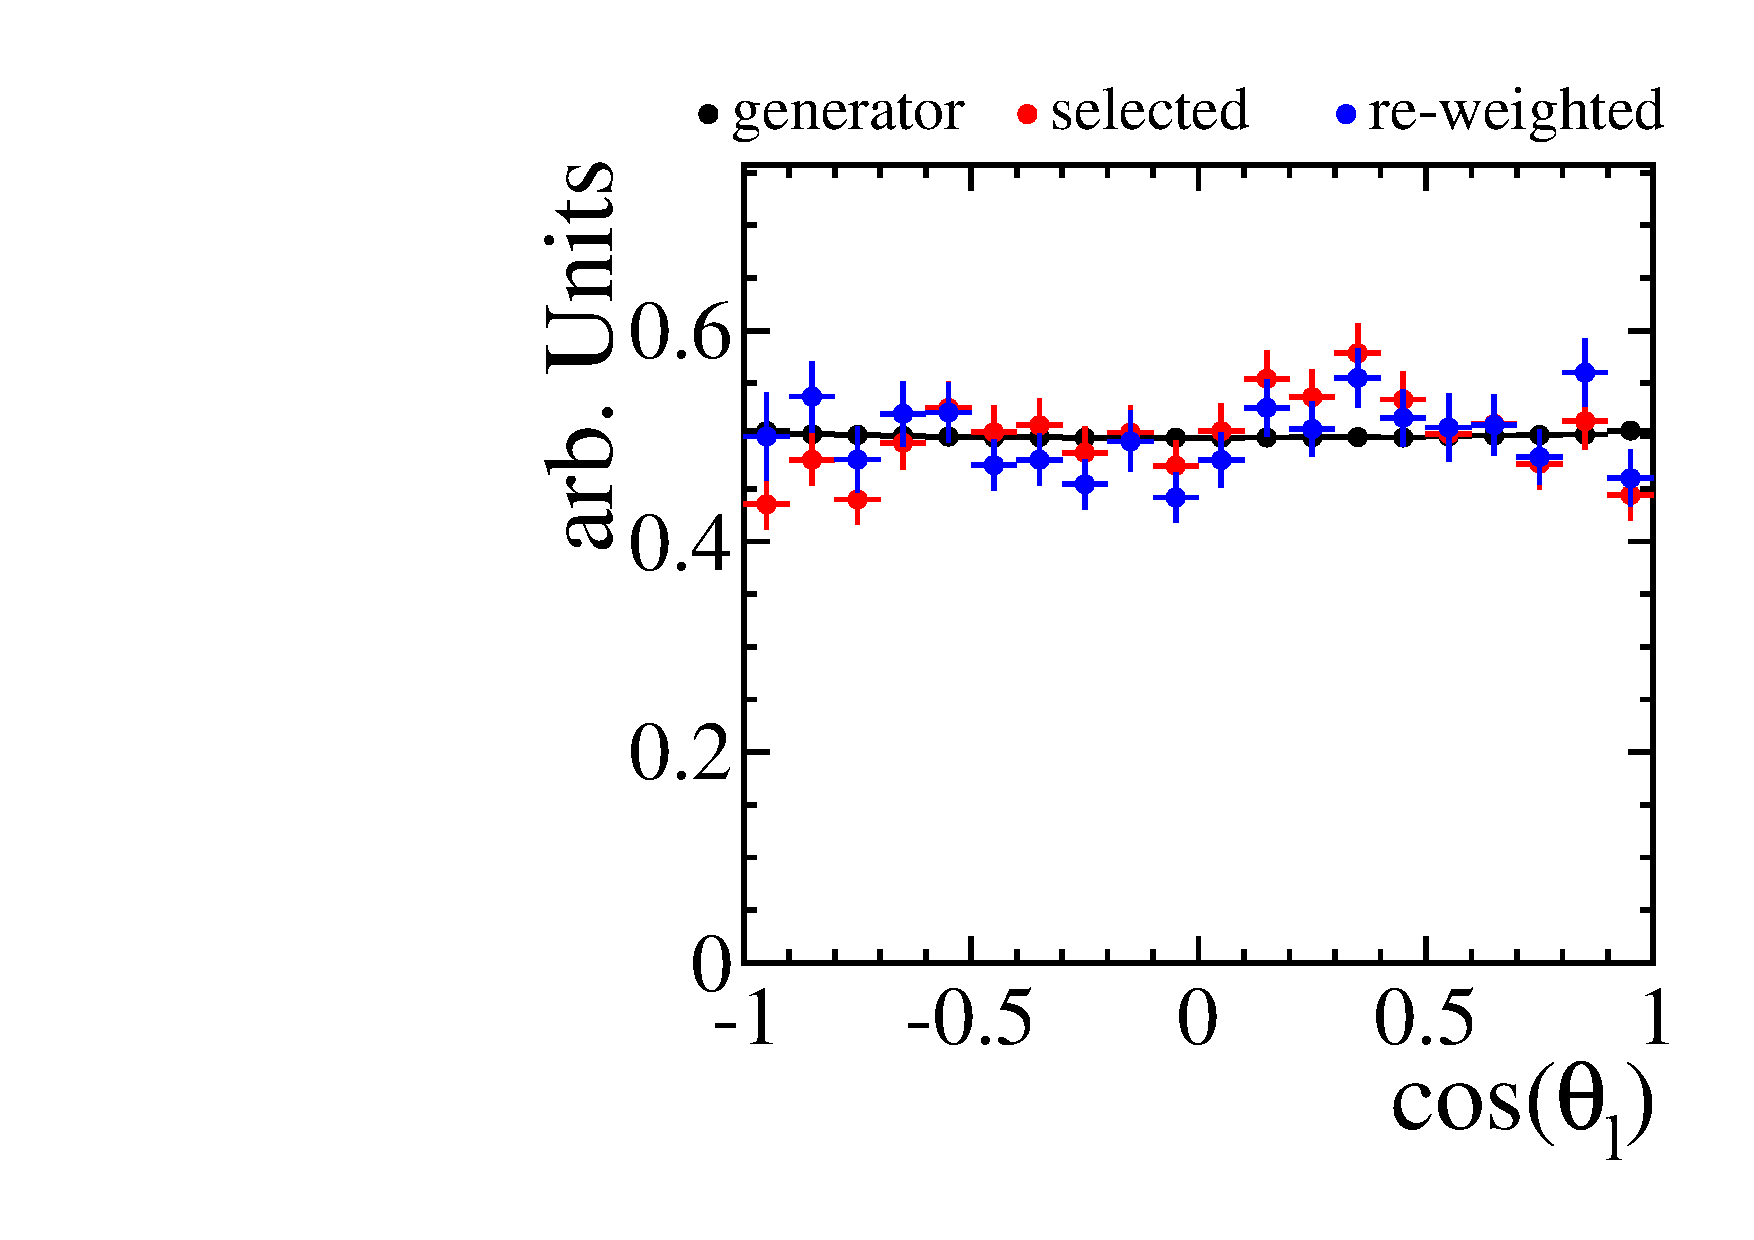
\includegraphics[width=0.48\columnwidth]{chapter5/figs/ac2/CorrectionsWithGen_ThetaL_new.pdf}}
\subfigure[]{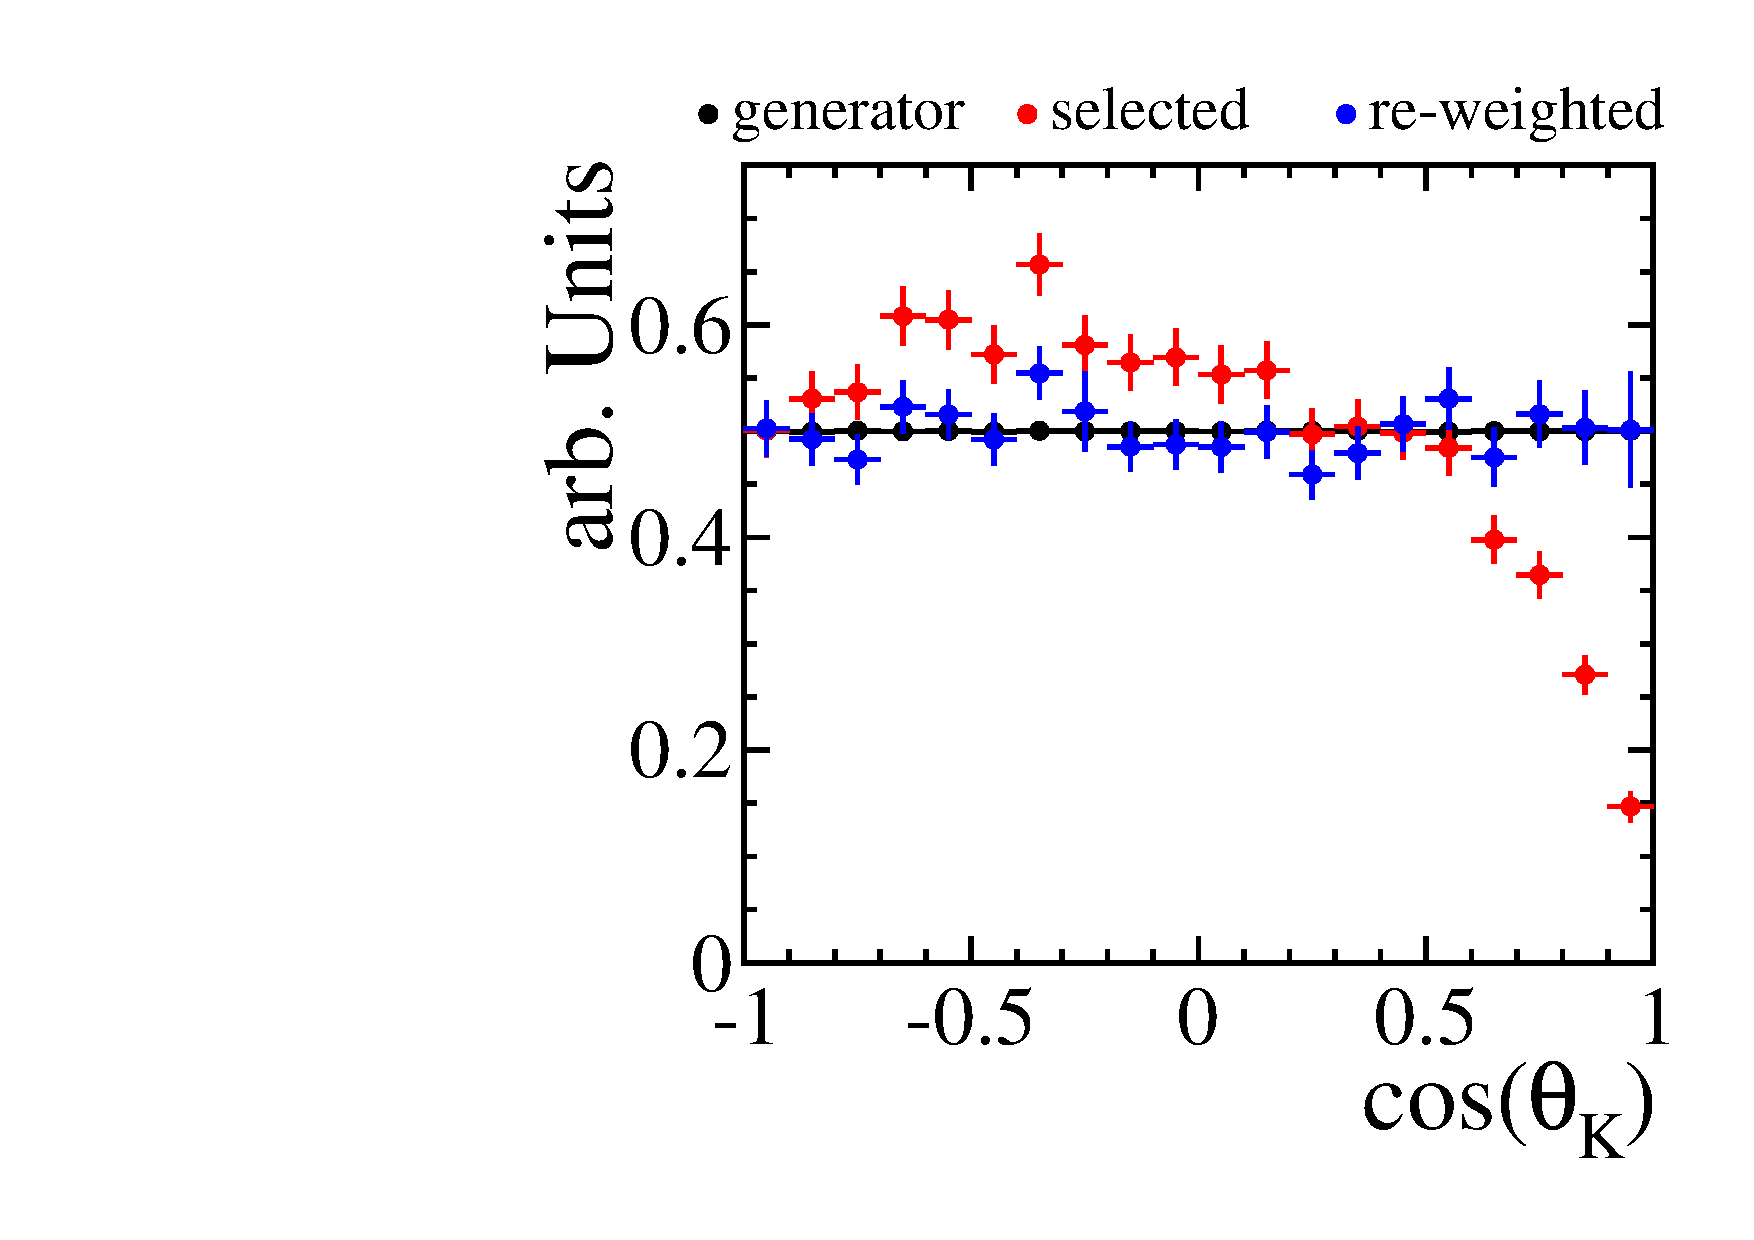
\includegraphics[width=0.48\columnwidth]{chapter5/figs/ac2/CorrectionsWithGen_ThetaK_new.pdf}}
\subfigure[]{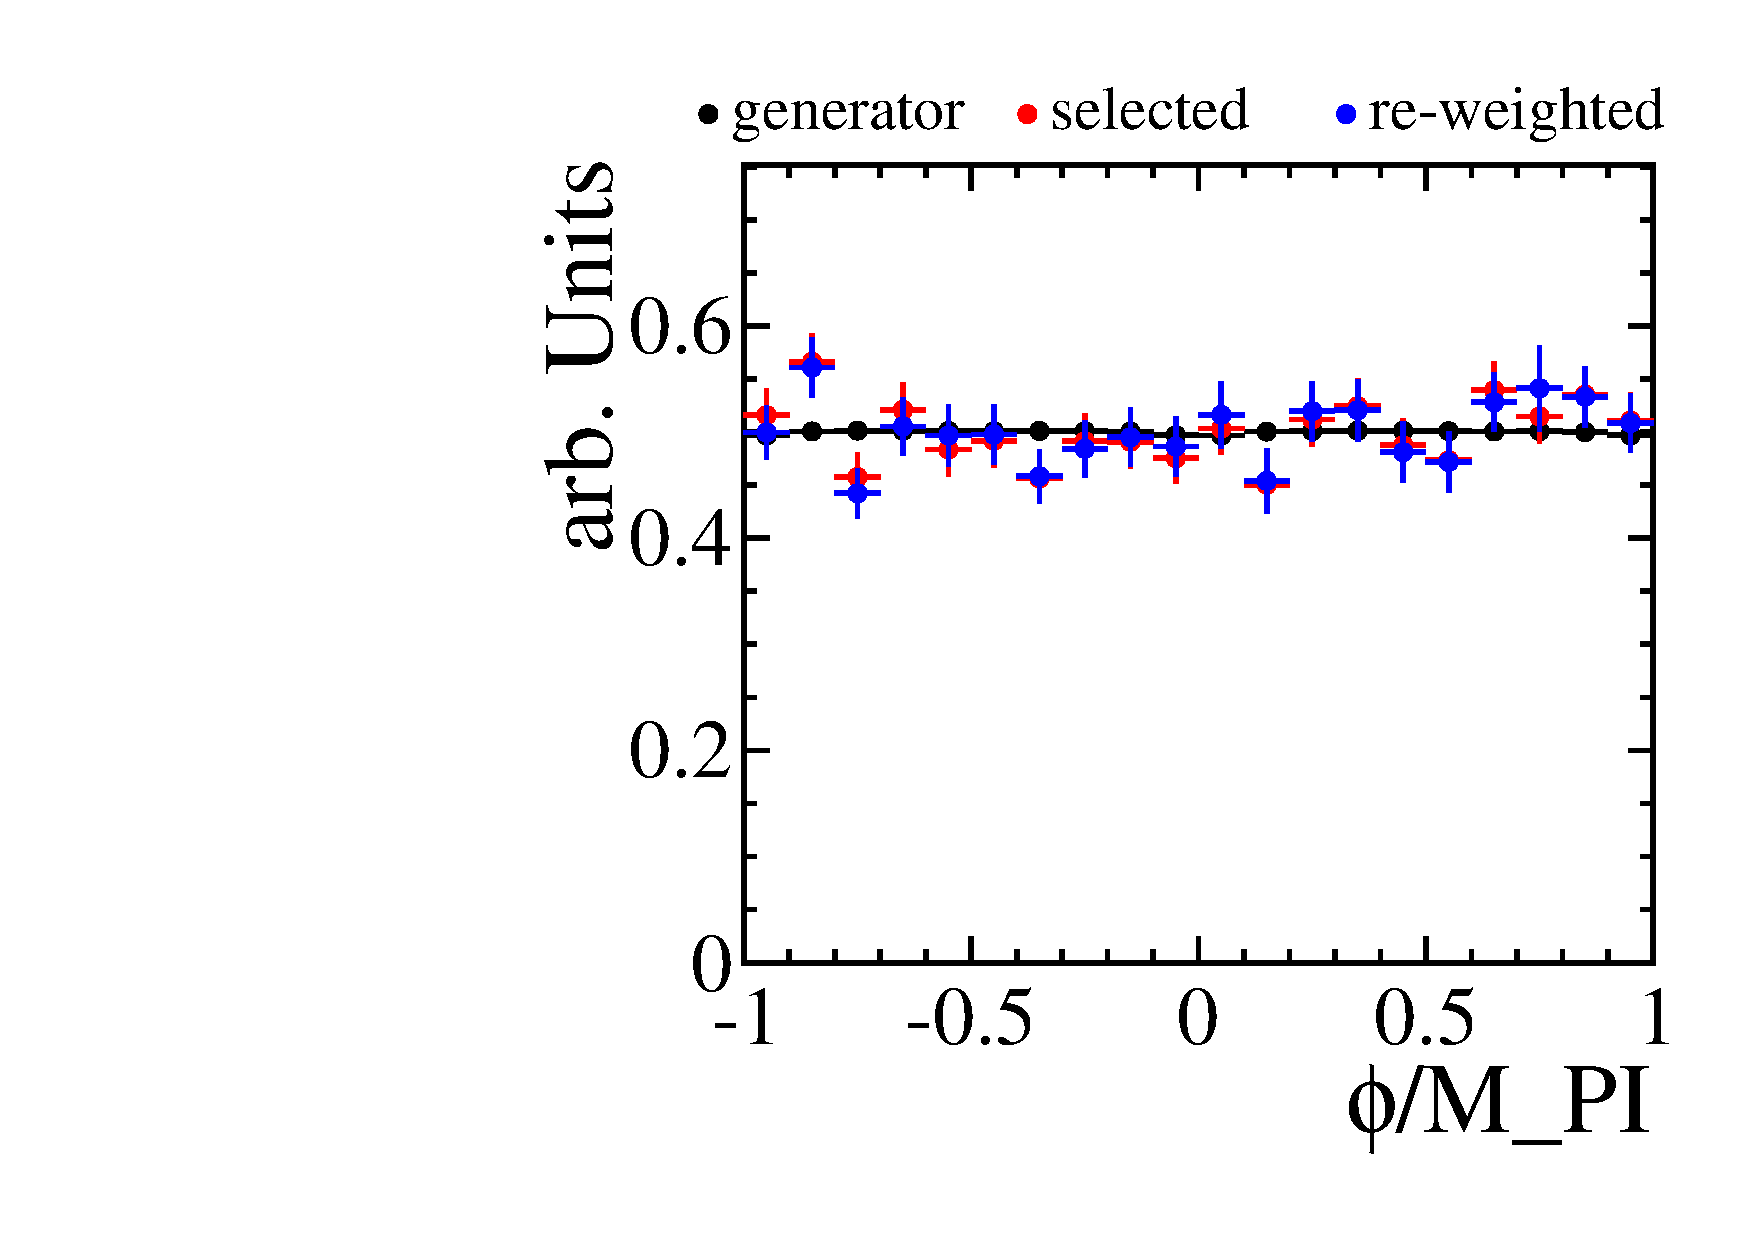
\includegraphics[width=0.48\columnwidth]{chapter5/figs/ac2/CorrectionsWithGen_Phi_new.pdf}}
\caption{Generated (black), offline selected (red) and re-weighted (blue) events for  \BdToKstmm using the factorised acceptance correction method.~\label{fig:corrphsp2}}
\end{figure}
The compatibility between the re-weighted distribution and the distribution  of generator level events 
is good for both acceptance correction methods.


The k-nearest-neighbour method is by construction the most optimal acceptance correction method as it relies only on the accuracy of the simulation
 from which to calculate the efficiency. 
However, the dependence on the simulation statistics in regions of phase
space with low efficiency does not allow it to be used with larger
datasets. The factorised efficiency correction has for the 1.0\invfb
analysis a lower total systematic error. The statistical component from
the simulation sample size is much smaller but the assumption of
factorisation incurs an additional but still small systematic uncertainty.

